\documentclass[10pt]{article}
\usepackage{graphicx} % Required for inserting images
\usepackage[a4paper,margin=2.2cm]{geometry}
\usepackage[ruled,vlined,linesnumbered]{algorithm2e}
\usepackage[T1]{fontenc}
\usepackage[utf8]{inputenc}
\usepackage{lmodern}
\usepackage{longtable}
\usepackage{microtype}
\usepackage{amsmath,amssymb,mathtools}
\usepackage{booktabs,tabularx,array,multirow}
\usepackage{enumitem}
\usepackage{appendix}
\usepackage{booktabs}
\usepackage{array}
\usepackage{xcolor}
\usepackage{tikz}
\usepackage{enumitem}
\usepackage{amsthm}
\usetikzlibrary{arrows.meta,
	positioning,
	fit,
	shapes.geometric, 
	backgrounds, 
	calc}
\usepackage{listings}
\usepackage{hyperref}
\usepackage[nameinlink,noabbrev]{cleveref}
\usepackage{caption}
\usepackage{subcaption}
\usepackage{url}
\usepackage{balance}
\usepackage{tabularx}
\usepackage{booktabs}
\usepackage{array}
\usepackage{makecell}
\usepackage{ragged2e}
\newcolumntype{C}[1]{>{\Centering\arraybackslash}p{#1}}
\newcolumntype{Y}{>{\RaggedRight\arraybackslash}X}

\definecolor{acmblue}{RGB}{37,80,130}
\definecolor{acmgray}{RGB}{245,247,249}
\definecolor{passgreen}{RGB}{34,139,34}
\definecolor{deviationorange}{RGB}{210,105,30}
\definecolor{skipgray}{RGB}{105,105,105}
\definecolor{failred}{RGB}{178,34,34}
\definecolor{alertred}{RGB}{178,34,34}
\definecolor{preservedgreen}{RGB}{34,139,34}
\definecolor{approximatedorange}{RGB}{210,105,30}
\definecolor{unsupportedgray}{RGB}{105,105,105}
\hypersetup{
	colorlinks=true,
	linkcolor=acmblue,
	citecolor=acmblue,
	urlcolor=acmblue,
	pdftitle={Agentic Configuration Management},
	pdfauthor={AUTHOR NAME}
}

\lstdefinestyle{acmcode}{
	basicstyle=\ttfamily\small,
	backgroundcolor=\color{acmgray},
	frame=single,
	rulecolor=\color{black!15},
	breaklines=true,
	columns=fullflexible,
	showstringspaces=false
}

\newcommand{\acmcore}{\textsc{ACM Core}}
\newcommand{\framework}{framework-independent}
\newcommand{\todo}[1]{\textcolor{red}{[TODO: #1]}}
\newcommand{\system}{\mathcal{S}}
\newcommand{\configgraph}{G_C}
\newcommand{\runtimegraph}{G_R}
\newcommand{\assurancegraph}{G_A}
\newcommand{\evolutiongraph}{G_E}
\newcommand{\statuspass}{\textcolor{passgreen}{\texttt{pass}}}
\newcommand{\statusdeviation}{\textcolor{deviationorange}{\texttt{pass\_with\_deviation}}}
\newcommand{\statusskip}{\textcolor{skipgray}{\texttt{skipped}}}
\newcommand{\statusfail}{\textcolor{failred}{\texttt{fail}}}
\newcommand{\statusnotexec}{\texttt{not\_executed}}
\newcommand{\statuspreserved}{\textcolor{preservedgreen}{\texttt{preserved}}}
\newcommand{\statusapproximated}{\textcolor{approximatedorange}{\texttt{approximated}}}
\newcommand{\statusunsupported}{\textcolor{unsupportedgray}{\texttt{unsupported}}}

\newtheorem{theorem}{Theorem}
\newtheorem{lemma}{Lemma}
\newtheorem{proposition}{Proposition}

\title{\textbf{Agentic Configuration Management (ACM):\\A Reference Configuration Model for Governed Agentic Systems}}

\author{
	Audrey Quessadda-Vial\\
	PwC\\
	\texttt{audrey.quessada-vial@pwc.com}
}

\date{Draft --- August 2026}

\begin{document}
	
	\maketitle
	
	
\section{Governance Semantics}
\label{sec:governance_semantics}
	
	The ACM reference model specifies the structural organization of governed agentic systems. This section complements the metamodel by defining the operational semantics governing lifecycle evolution, state evaluation, dependency propagation, and runtime reconstruction.
	
	The governance semantics are intentionally defined independently from any execution framework. Their purpose is not to describe execution behavior but to provide a deterministic interpretation of governed configurations throughout their lifecycle.
	
	Let
	
	\begin{equation}
		G=(V,E)
		\label{eq:configuration_graph}
	\end{equation}
	
	denote the ACM Configuration Graph introduced in Section~\ref{sec:configuration_graph}, where each vertex represents an immutable ACI revision and each edge represents a typed governance relationship.
	
	Each revision is associated with a governance descriptor
	
	\begin{equation}
		\Gamma(v)=
		\left(
		L(v),
		Q(v),
		A(v),
		I(v),
		El(v),
		Rt(v)
		\right),
		\label{eq:governance_descriptor}
	\end{equation}
	
	where the individual components respectively denote the lifecycle, quality, assurance, impact, eligibility, and runtime states associated with revision $v$.
	
	The governance descriptor is a logical representation of the governance status of an ACI revision. It does not perform any computation itself. Individual state components are evaluated independently according to the semantics introduced in the following subsections and are subsequently propagated through governance relationships according to explicitly defined propagation policies.
	
	This separation between state spaces, evaluation functions, propagation policies, and runtime reconstruction ensures that each semantic component is defined once and reused consistently throughout the model.
	
	\subsection{Governance Lifecycle}
	\label{sec:lifecycle_semantics}
	
	The lifecycle dimension represents the intrinsic governance maturity of an immutable ACI revision independently of any dependency or runtime consideration. Unlike the remaining governance dimensions, lifecycle states are explicitly assigned through governance actions rather than derived by propagation.
	
	Figure~\ref{fig:lifecycle_state_machine} presents the lifecycle state machine associated with every ACI revision.
	
	Each revision progresses monotonically through the lifecycle. Once a revision reaches a given state, it cannot transition back to a previous lifecycle state.
	
	This monotonic property guarantees configuration immutability while preserving complete governance traceability across successive revisions.
	
	Lifecycle transitions are therefore constrained by a partial order
	
	\begin{equation}
		Draft
		<
		Validated
		<
		Approved
		<
		Released
		<
		Deprecated
		<
		Archived,
		\label{eq:lifecycle_order}
	\end{equation}
	
	where each transition represents an explicit governance decision.
	
	The lifecycle state is denoted
	
	\begin{equation}
		L(v)\in\mathcal{L},
		\label{eq:lifecycle_state}
	\end{equation}
	
	where $\mathcal{L}$ denotes the lifecycle state space formally defined in Appendix~\ref{appendix:lifecycle}.
	
	Unlike derived governance dimensions introduced later in this section, lifecycle states never result from dependency propagation. They constitute primary governance information from which eligibility and propagation decisions are subsequently derived.
	
	\subsection{Governance State Spaces}
	\label{sec:governance_state_spaces}
	
	The governance semantics are defined over six orthogonal state spaces describing complementary aspects of an immutable ACI revision. Each state space captures an independent governance concern and is evaluated according to its own semantics.
	
	Unlike the lifecycle state, which is explicitly assigned through governance decisions, the remaining dimensions are either derived from governance evidence, dependency analysis, or runtime observations.
	
	Figure~\ref{fig:governance_state_machine} summarizes the six orthogonal state machines used throughout the remainder of this paper.
	
	The governance dimensions are:
	
	\begin{itemize}
		\item \textbf{Lifecycle ($\mathcal{L}$):} governance maturity of a revision;
		\item \textbf{Quality ($\mathcal{Q}$):} validation status of the revision itself;
		\item \textbf{Assurance ($\mathcal{A}$):} completeness of governance evidence;
		\item \textbf{Impact ($\mathcal{I}$):} propagation status resulting from dependency analysis;
		\item \textbf{Eligibility ($\mathcal{E}$):} authorization for operational use;
		\item \textbf{Runtime ($\mathcal{R}$):} observed execution state.
	\end{itemize}
	
	Each state space is formally defined in Appendix~\ref{appendix:state_spaces}. Their interaction is specified later through evaluation functions and the propagation operator.
	
	\subsection{Propagation Policies}
	\label{sec:propagation_policies}
	
	Governance propagation is intentionally separated from state evaluation. While governance state spaces define \emph{what} is evaluated, propagation policies define \emph{how} governance information is allowed to traverse configuration relationships.
	
	Each relationship type is therefore associated with a propagation policy determining the effect of governance changes on dependent revisions. Policies are intrinsic properties of relationship types and remain independent of the current governance states of the connected revisions.
	
	A propagation policy is defined as a mapping
	
	\begin{equation}
		\Pi : T_R \rightarrow \mathcal{P},
		\label{eq:policy_mapping}
	\end{equation}
	
	where $T_R$ denotes the set of relationship types introduced by the reference model and $\mathcal{P}$ is the finite set of propagation policies
	
	\begin{equation}
		\mathcal{P}=
		\left\{
		\textit{Blocking},
		\textit{Warning},
		\textit{Informational},
		\textit{None}
		\right\}.
		\label{eq:policy_space}
	\end{equation}
	
	Each policy specifies the governance significance of a relationship during propagation.
	
	\begin{itemize}
		\item \textbf{Blocking} indicates that governance changes affecting the source revision shall propagate to dependent revisions and may restrict their operational eligibility until reassessment is completed.
		
		\item \textbf{Warning} propagates governance information without automatically preventing operational use. The affected revision remains executable but requires governance attention.
		
		\item \textbf{Informational} records the dependency for traceability purposes without modifying governance states.
		
		\item \textbf{None} disables propagation across the relationship while preserving the structural dependency.
	\end{itemize}
	
	Propagation policies are associated with relationship types rather than individual revisions. Consequently, identical relationship types always induce identical propagation semantics independently of the connected ACI revisions.
	
	When several propagation paths converge on the same revision, multiple propagation policies may simultaneously apply. Their combined effect is resolved deterministically according to the precedence rules defined in Appendix~\ref{appendix:propagation_policies}. This deterministic composition guarantees that governance propagation remains independent of traversal order.
	
	\subsection{Governance Evaluation Functions}
	\label{sec:evaluation_functions}
	
	The governance state spaces introduced previously define the possible states associated with an ACI revision. Governance evaluation functions determine how these states are assigned from governance evidence while remaining independent of dependency propagation.
	
	Three evaluation functions are defined. They respectively evaluate intrinsic quality, governance assurance, and operational eligibility. Each function produces a deterministic result for a given governance context and is evaluated independently before any propagation mechanism is applied.
	
	\subsubsection{Quality Evaluation}
	
	The quality evaluation function assigns the quality state associated with an ACI revision according to the available validation evidence.
	
	\begin{equation}
		f_{\mathrm{quality}} : V \rightarrow \mathcal{Q},
		\label{eq:f_quality}
	\end{equation}
	
	where $V$ denotes the set of ACI revisions and $\mathcal{Q}$ is the quality state space introduced in Section~\ref{sec:governance_state_spaces}.
	
	The resulting quality state is denoted
	
	\begin{equation}
		Q(v)=f_{\mathrm{quality}}(v).
		\label{eq:quality_assignment}
	\end{equation}
	
	Quality evaluation depends exclusively on the considered revision and is therefore independent of dependency propagation.
	
	\subsubsection{Assurance Evaluation}
	
	The assurance evaluation function determines the completeness of governance evidence associated with a revision.
	
	\begin{equation}
		f_{\mathrm{assurance}} : V \rightarrow \mathcal{A},
		\label{eq:f_assurance}
	\end{equation}
	
	where $\mathcal{A}$ denotes the assurance state space.
	
	The resulting assurance state is
	
	\begin{equation}
		A(v)=f_{\mathrm{assurance}}(v).
		\label{eq:assurance_assignment}
	\end{equation}
	
	Assurance reflects the completeness of governance evidence independently of the intrinsic quality of the revision.
	
	\subsubsection{Eligibility Evaluation}
	
	Operational eligibility depends on the combined interpretation of the governance dimensions. Unlike quality and assurance, eligibility is therefore derived from multiple governance states.
	
	The eligibility evaluation function is defined as
	
	\begin{equation}
		f_{\mathrm{elig}} :
		\mathcal{L}
		\times
		\mathcal{Q}
		\times
		\mathcal{A}
		\times
		\mathcal{I}
		\times
		\mathcal{P}
		\rightarrow
		\mathcal{E},
		\label{eq:f_elig}
	\end{equation}
	
	where $\mathcal{P}$ denotes the propagation policy space defined in Section~\ref{sec:propagation_policies}.
	
	The eligibility state associated with revision $v$ is therefore
	
	\begin{equation}
		El(v)=
		f_{\mathrm{elig}}
		\left(
		L(v),
		Q(v),
		A(v),
		I(v),
		\Pi
		\right).
		\label{eq:eligibility_assignment}
	\end{equation}
	
	Eligibility summarizes the governance status required for operational use. The evaluation itself remains local to the considered revision. Dependency propagation and the computation of effective governance states are introduced separately in the following subsection.
	
	\subsection{Propagation Semantics}
	\label{subsec:propagation_semantics}
	
	The governance dimensions introduced in the previous subsections define the
	local state associated with each ACI revision. Governance evaluation, however,
	cannot be performed independently for each revision because configuration
	dependencies may propagate the consequences of a local change throughout the
	configuration graph. The propagation semantics therefore define how governance
	states are iteratively updated until a globally consistent evaluation is
	reached.
	
	Propagation follows the directed relationships of the configuration graph and
	is controlled by the propagation policies introduced in
	Section~\ref{subsec:propagation_policies}. These policies determine whether a
	relationship blocks propagation, propagates a warning, carries informational
	effects only, or does not participate in governance propagation.
	
	The propagation process is defined by a global operator,
	denoted $\mathrm{Prop}$, which applies the propagation policies over the
	configuration graph and updates the impact state of affected revisions.
	Evaluation functions introduced in the previous subsection are subsequently
	applied locally to derive the resulting governance states.
	
	Formally, let
	
	\begin{equation}
		\label{eq:prop_operator}
		\mathrm{Prop} :
		G \times \Pi
		\rightarrow
		G,
	\end{equation}
	
	where $G$ denotes the governed configuration graph and $\Pi$ the propagation
	policy associated with each relationship type.
	
	Starting from an initial governance state, successive applications of
	$\mathrm{Prop}$ generate the sequence
	
	\begin{equation}
		\label{eq:prop_iteration}
		G^{(k+1)}
		=
		\mathrm{Prop}
		\!\left(
		G^{(k)},
		\Pi
		\right),
	\end{equation}
	
	where $k$ denotes the propagation iteration.
	
	Propagation terminates when the governance state becomes stable, that is, when
	an additional application of the operator no longer modifies any propagated
	state.
	
\begin{equation}
	\label{eq:fixed_point}
	\mathrm{Prop}_{G,\Pi}
	\!\left(
	\iota^{*}
	\right)
	=
	\iota^{*}.
\end{equation}

The stabilized impact valuation $\iota^{*}$ is the \emph{least fixed point} of
the propagation semantics and provides the propagated impact state used by the
subsequent local governance evaluation.
	
Because impact propagation is performed before eligibility evaluation, the eligibility of each revision remains a purely local computation.
Once the propagated impact state has stabilized, the eligibility state is obtained by applying the evaluation function defined in
Section~\ref{subsec:governance_evaluation} to the final governance descriptor associated with each revision.
	
The propagation semantics are independent of any implementation strategy.
A compliant implementation may therefore employ different execution algorithms, provided that they compute the same least fixed point. The reference implementation adopts a worklist-based evaluation strategy because it avoids re-evaluating unaffected revisions while preserving the normative semantics. The complete worklist algorithm, together with the proofs of monotonicity, termination, convergence, and uniqueness of the least fixed point, is provided in Appendix~A.5.
	
	
	%%%%%%%%%%%%%%%%%%%%%%%%%%%%%%%%%%%%%%%%%%%%%%%%%%%%%%%%%%%%%%%%%%%%%%%%%%%%%%%%
	\subsubsection{Unified Governance State Diagram}
	
	Figure~\ref{fig:governance_state_machine} illustrates the interaction between
	the lifecycle state and the four orthogonal governance state machines.
	
	%===============================================================================
	% TikZ placeholder
	%
	% The figure shall represent:
	%
	% - Lifecycle chain:
	%   Draft -> Review -> Validated -> Approved -> Deprecated -> Archived
	%
	% - Four independent state machines:
	%     Quality
	%     Impact
	%     Assurance
	%     Eligibility
	%
	% - Evaluation function:
	%
	%      (L,Q,A,I) ---> Eligibility
	%
	% IEEE academic style.
	%
	%===============================================================================
	
	\begin{figure*}[t]
		\centering
		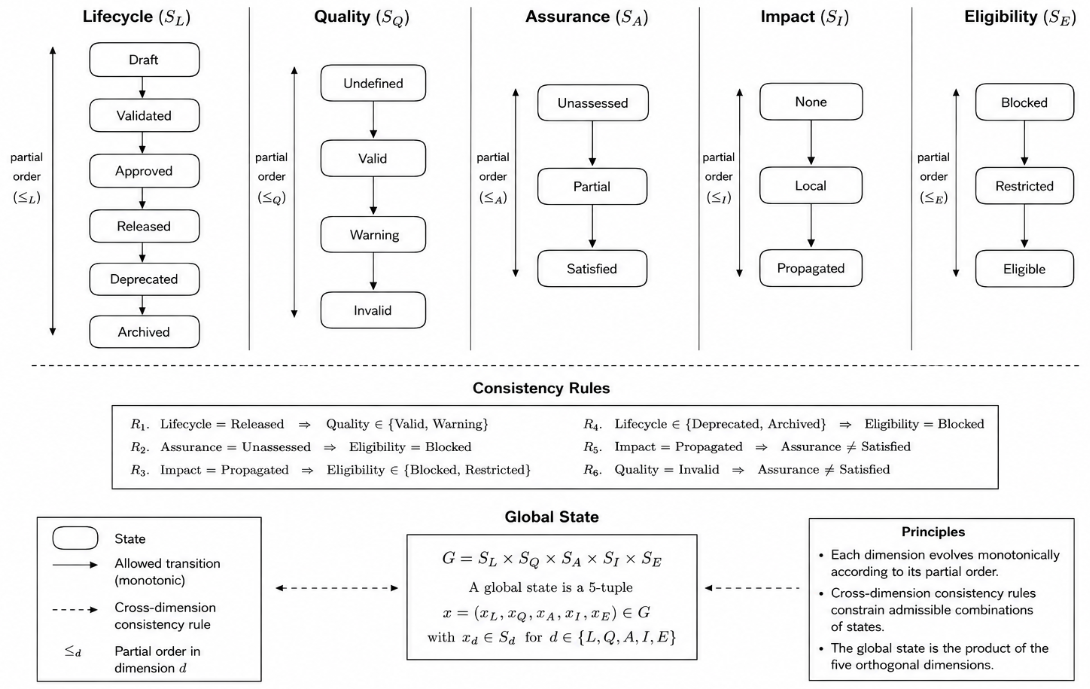
\includegraphics[width=\textwidth]{figures/othogonal_governance_state_machine.png}
		
		\caption{Orthogonal governance state machines composing the ACM governance
			semantics. Lifecycle, quality, impact, and assurance are evaluated as distinct
			state dimensions, while execution eligibility is derived through the evaluation
			function $f(L,Q,A,I)$.}
		\label{fig:governance_state_machine}
	\end{figure*}
	
	%%%%%%%%%%%%%%%%%%%%%%%%%%%%%%%%%%%%%%%%%%%%%%%%%%%%%%%%%%%%%%%%%%%%%%%%%%%%%%%%
	\subsubsection{Transition Properties}
	
	The governance state machines satisfy the following properties.
	
	\paragraph{Property G1 (Determinism).}
	
	For every governance event, each state machine admits exactly one successor
	state.
	
	\paragraph{Property G2 (Orthogonality).}
	
	Each governance dimension evolves independently according to its own transition
	function (see Appendix section ~\ref{appendix:governance_orthogonality}).
	
	\paragraph{Property G3 (Composability).}
	
	The global governance state is obtained through the composition of independent
	semantic dimensions rather than by constructing a single global automaton.
	
	\paragraph{Property G4 (Extensibility).}
	
	Additional governance dimensions may be introduced without modifying the
	existing state machines provided that they expose well-defined evaluation
	functions.
	
	These properties considerably simplify future extensions of ACM while
	preserving backward compatibility of governance semantics.
	
	The next subsection formalizes how local governance changes propagate through
	dependency relationships, enabling global reasoning over complete agentic
	configuration graphs.
	
	Figure~\ref{fig:impact_propagation} illustrates the propagation of a local
	configuration change through governance dependencies. The directly modified
	revision receives the \textit{Local} impact state, while reachable dependent
	revisions receive the \textit{Propagated} state. Revisions outside the
	resulting impact closure remain in the \textit{None} state.
	
	\begin{figure*}[t]
		\centering
		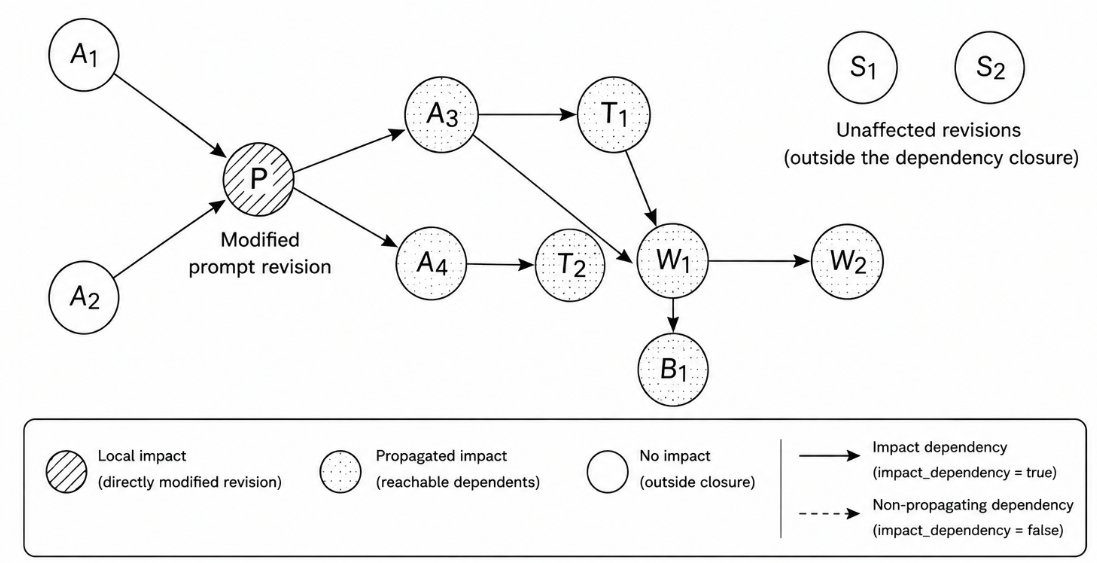
\includegraphics[width=\textwidth]{figures/Impact_propagation_revision.png}
		\caption{
			Impact propagation following the modification of prompt revision $P$.
			The directly modified revision receives a local impact state, while
			reachable dependent revisions receive a propagated impact state.
			Revisions outside the dependency closure remain unaffected.
		}
		\label{fig:impact-propagation}
	\end{figure*}
	
	%%%%%%%%%%%%%%%%%%%%%%%%%%%%%%%%%%%%%%%%%%%%%%%%%%%%%%%%%%%%%%%%%%
	\subsubsection{Illustrative Example}
	
	Assume that a workflow
	
	\[
	W
	\]
	
	contains an agent
	
	\[
	A_1
	\]
	
	whose prompt revision is modified. The prompt immediately becomes
	
	\[
	Local.
	\]
	
	The associated agent, workflow, runtime deployment, and assurance reports become:
	
	\[
	Propagated,
	\]
	
	because each depends on the modified configuration revision.
	
	Importantly, propagation alone does not imply execution failure.
	
	It merely indicates that governance evaluation should be recomputed before the
	corresponding artifacts are considered trustworthy.
	
	Figure~\ref{fig:agent_state_before_after} illustrates the non-destructive
	propagation of governance state for a single agent. A change to a required
	prompt revision does not modify the agent revision or its intrinsic lifecycle
	and quality states. Instead, the propagation process recalculates the agent's
	impact, assurance, and eligibility states from the updated dependency context.
	\begin{figure*}[t]
		\centering
		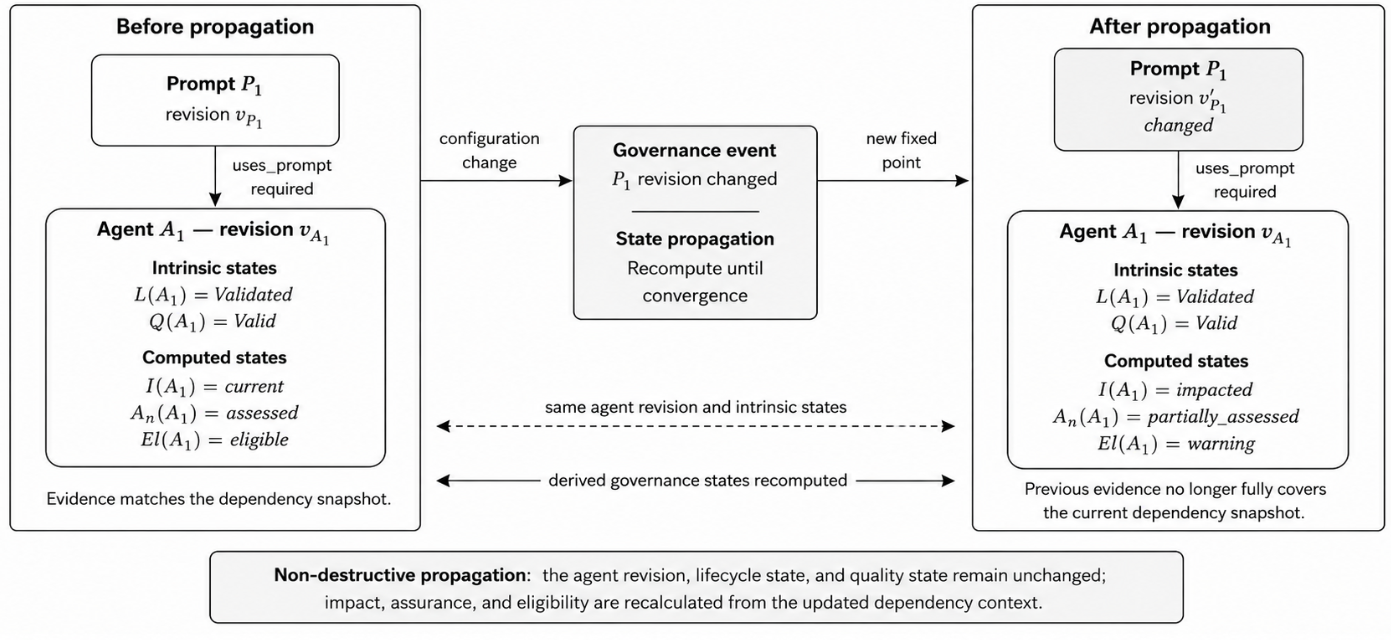
\includegraphics[width=\textwidth]{figures/non_destructive_state_propagation.png}
		
		\caption{Non-destructive governance state propagation for an agent. A change
			to a required prompt revision preserves the agent revision and its intrinsic
			lifecycle and quality states, while the derived impact, assurance, and
			eligibility states are recomputed from the updated dependency context.}
		\label{fig:agent_state_before_after}
	\end{figure*}
	
	%%%%%%%%%%%%%%%%%%%%%%%%%%%%%%%%%%%%%%%%%%%%%%%%%%%%%%%%%%%%%%%%%%%%%%%%%%%%%%%
	
	This fixed-point formulation establishes the formal semantics of governance
	propagation independently of any particular implementation. Whether ACM is
	implemented through recursive graph traversal, work-list evaluation, or
	incremental update algorithms, every compliant implementation is required to
	compute the same least fixed point, thereby guaranteeing deterministic,
	reproducible, and implementation-independent governance evaluation.
	%%%%%%%%%%%%%%%%%%%%%%%%%%%%%%%%%%%%%%%%%%%%%%%%%%%%%%%%%%%%%%%%%%%%%%%%%%%%%%%%
	\subsubsection{Illustrative Example}
	
	Figure~\ref{fig:governance_propagation} illustrates the propagation of a prompt
	deprecation through an agentic configuration. The prompt revision becomes
	\texttt{deprecated}; the dependent agent becomes \texttt{impacted}; its
	effective assurance is downgraded to
	\texttt{partial}; and its eligibility changes from
	\texttt{eligible} to
	\texttt{warning}. Importantly, neither the lifecycle nor the declared quality
	of the agent is modified. This example illustrates the central principle of ACM
	that governance propagation affects derived governance states rather than
	intrinsic configuration properties.
	
	%%%%%%%%%%%%%%%%%%%%%%%%%%%%%%%%%%%%%%%%%%%%%%%%%%%%%%%%%%%%%%%%%%%%%%%%%%%%%%%%
	% Figure to be inserted here
	%
	% Figure:
	% Governance State Propagation
	%
	% (TikZ IEEE academic style)
	%
	%%%%%%%%%%%%%%%%%%%%%%%%%%%%%%%%%%%%%%%%%%%%%%%%%%%%%%%%%%%%%%%%%%%%%%%%%%%%%%%%
	% Figure: Governance State Propagation
	%%%%%%%%%%%%%%%%%%%%%%%%%%%%%%%%%%%%%%%%%%%%%%%%%%%%%%%%%%%%%%%%%%%%%%%%%%%%%%%%
	\begin{figure}[t]
		\centering
		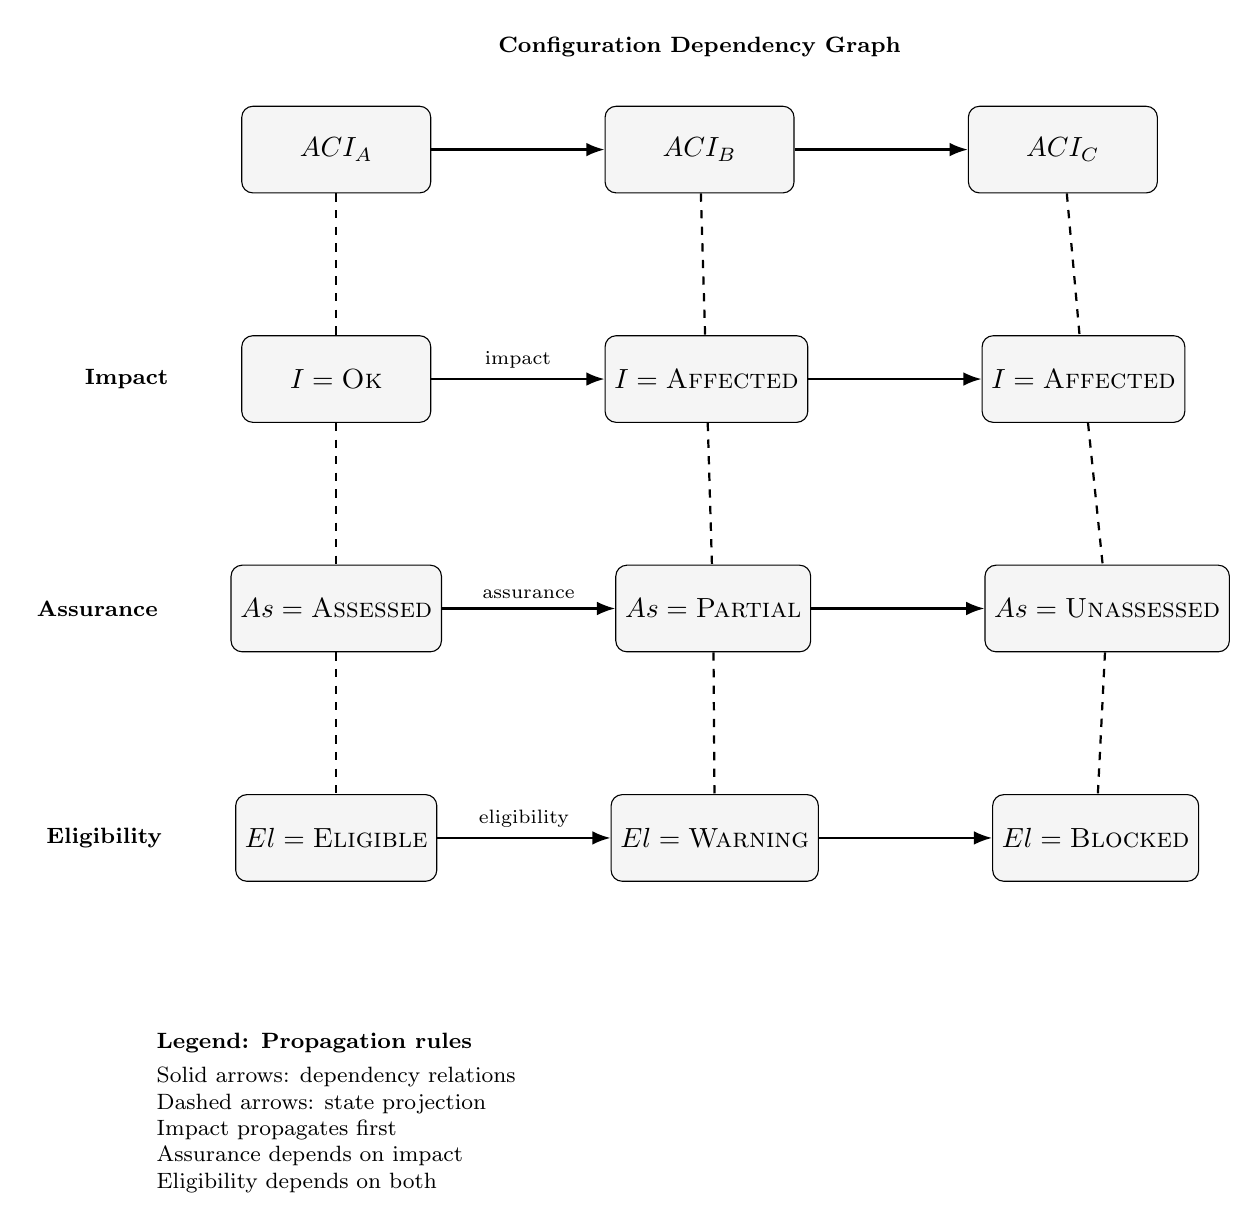
\begin{tikzpicture}[
			>=Latex,
			node distance=18mm and 22mm,
			aci/.style={
				draw,
				rounded corners,
				minimum width=24mm,
				minimum height=11mm,
				align=center,
				fill=gray!8
			},
			flow/.style={
				->,
				thick
			},
			prop/.style={
				dashed,
				thick
			},
			annot/.style={
				font=\footnotesize,
				align=center
			}
			]
			
			%-------------------------------------------------
			% Configuration graph
			%-------------------------------------------------
			
			\node[aci] (A) {$ACI_A$};
			\node[aci,right=of A] (B) {$ACI_B$};
			\node[aci,right=of B] (C) {$ACI_C$};
			
			\draw[flow] (A)--(B);
			\draw[flow] (B)--(C);
			
			\node[annot,above=5mm of B]
			{\textbf{Configuration Dependency Graph}};
			
			%-------------------------------------------------
			% Impact propagation
			%-------------------------------------------------
			
			\node[aci,below=18mm of A] (IA) {$I=\textsc{Ok}$};
			\node[aci,right=of IA] (IB) {$I=\textsc{Affected}$};
			\node[aci,right=of IB] (IC) {$I=\textsc{Affected}$};
			
			\draw[prop] (A)--(IA);
			\draw[prop] (B)--(IB);
			\draw[prop] (C)--(IC);
			
			\draw[flow] (IA)--node[above,font=\scriptsize]{impact}(IB);
			\draw[flow] (IB)--node[above,font=\scriptsize]{}(IC);
			
			\node[annot,left=8mm of IA]
			{\textbf{Impact}};
			
			%-------------------------------------------------
			% Assurance propagation
			%-------------------------------------------------
			
			\node[aci,below=18mm of IA] (AA) {$As=\textsc{Assessed}$};
			\node[aci,right=of AA] (AB) {$As=\textsc{Partial}$};
			\node[aci,right=of AB] (AC) {$As=\textsc{Unassessed}$};
			
			\draw[prop] (IA)--(AA);
			\draw[prop] (IB)--(AB);
			\draw[prop] (IC)--(AC);
			
			\draw[flow] (AA)--node[above,font=\scriptsize]{assurance}(AB);
			\draw[flow] (AB)--(AC);
			
			\node[annot,left=8mm of AA]
			{\textbf{Assurance}};
			
			%-------------------------------------------------
			% Eligibility propagation
			%-------------------------------------------------
			
			\node[aci,below=18mm of AA] (EA) {$El=\textsc{Eligible}$};
			\node[aci,right=of EA] (EB) {$El=\textsc{Warning}$};
			\node[aci,right=of EB] (EC) {$El=\textsc{Blocked}$};
			
			\draw[prop] (AA)--(EA);
			\draw[prop] (AB)--(EB);
			\draw[prop] (AC)--(EC);
			
			\draw[flow] (EA)--node[above,font=\scriptsize]{eligibility}(EB);
			\draw[flow] (EB)--(EC);
			
			\node[annot,left=8mm of EA]
			{\textbf{Eligibility}};
			
			%-------------------------------------------------
			% Legend
			%-------------------------------------------------
			
			\node[
			align=left,
			below=18mm of EA,
			font=\footnotesize
			]
			{
				\textbf{Legend: Propagation rules}\\[1mm]
				Solid arrows: dependency relations\\
				Dashed arrows: state projection\\
				Impact propagates first\\
				Assurance depends on impact\\
				Eligibility depends on both
			};
			
		\end{tikzpicture}
		
		\caption{Governance state propagation across the configuration graph.
			A structural dependency first propagates impact, which subsequently influences
			assurance evaluation and finally execution eligibility. The three governance
			dimensions remain conceptually independent while being evaluated in a
			deterministic order.}
		\label{fig:governance_propagation}
	\end{figure}
	%%%%%%%%%%%%%%%%%%%%%%%%%%%%%%%%%%%%%%%%%%%%%%%%%%%%%%%%%%%%%%%%%%%%%%%%%%%%%%%%
	
	%%%%%%%%%%%%%%%%%%%%%%%%%%%%%%%%%%%%%%%%%%%%%%%%%%%%%%%%%%%%%%%%%%%%%%%%%%%%%%%%
	\subsection{Runtime Semantics}
	\label{subsec:runtime_semantics}
	
	The governance semantics defined so far describe how configuration states evolve
	within the immutable configuration graph. Runtime execution introduces an
	additional dimension that cannot be represented solely by static configuration
	artifacts. Agent executions create transient observations whose purpose is not
	to modify the governed configuration but to record how a released baseline is
	instantiated during execution.
	
	Accordingly, ACM distinguishes the \emph{Configuration Graph}, which contains
	immutable governed revisions, from the \emph{Runtime Graph}, which represents
	the execution state derived from a specific released baseline. Runtime
	observations never alter immutable configuration revisions. Instead, they are
	associated with the corresponding governed artifacts through stable revision
	identifiers and provenance relationships.
	
	The Runtime Graph is constructed from an ordered sequence of normalized runtime
	events. Each event captures an observable execution transition together with the
	identifier of the corresponding governed revision. Because runtime observations
	are represented independently from framework-specific execution traces, the same
	governance semantics can be applied to heterogeneous execution frameworks after
	semantic projection into the ACM reference model.
	
	Rather than storing successive runtime snapshots, ACM defines the runtime state
	as the result of replaying the normalized event sequence from a released
	baseline. Starting from the immutable configuration represented by the baseline,
	runtime events are deterministically applied in chronological order to
	reconstruct the Runtime Graph corresponding to any observation point.
	
	This separation provides two complementary benefits. First, released
	configurations remain immutable throughout execution, preserving configuration
	integrity and provenance. Second, runtime reconstruction becomes independent of
	the execution framework, provided that equivalent normalized events are
	available. Consequently, runtime analyses, governance verification, and
	conformance checking operate on a canonical Runtime Graph rather than on
	framework-specific execution representations.
	
	The replay semantics are intentionally defined independently of the propagation
	operator introduced in Section~\ref{sec:propagation_semantics}. Propagation
	computes the stabilized governance state associated with immutable
	configurations, whereas replay reconstructs the execution state generated from a
	released baseline. These two mechanisms therefore address complementary
	concerns: governance evaluation determines the valid configuration to be
	executed, while runtime replay reconstructs how that configuration was actually
	executed.
	
	The formal definition of normalized runtime events, the replay function, the
	incremental reconstruction procedure, and the associated correctness properties
	are presented in Appendix ~\ref{appendix:runtime_semantics}.
	
	\subsection{Formal Properties}
	\label{sec:formal_properties}
	
	The governance semantics defined in the previous subsections satisfy a number of
	formal properties that ensure the consistency, reproducibility, and
	predictability of ACM evaluations. These properties follow directly from the
	state spaces, evaluation functions, propagation semantics, and runtime replay
	model introduced throughout Section~5.
	
	First, the impact propagation semantics are monotone over the finite impact
	lattice defined in Appendix~A.3. Consequently, iterative propagation converges
	toward the least fixed point above the initial impact valuation, while the
	reference worklist algorithm computes the same stabilized result under any fair
	evaluation strategy. The corresponding proofs are provided in
	Appendix~A.6.
	
	Second, runtime replay is deterministic. Given an immutable released baseline
	and an identical ordered sequence of normalized runtime events, replay always
	reconstructs the same Runtime Graph. This property guarantees that runtime
	observations remain reproducible independently of the underlying execution
	framework after semantic projection into the ACM reference model. The formal
	replay model and proof of determinism are presented in Appendix~A.7.
	
	Together, these properties establish that governance evaluation and runtime
	reconstruction are reproducible and implementation-independent. For identical
	governed configurations and equivalent normalized runtime observations, ACM
	always produces identical governance states and identical reconstructed Runtime
	Graphs. This determinism provides the foundation for reproducible governance
	verification, impact analysis, runtime conformance checking, and assurance
	evaluation across heterogeneous agentic frameworks.
	
	The complete proofs, together with the complexity analysis and additional formal
	results, are presented in Appendix~A.8.
	
	
	
	
	
	
	
	
	
	
	
	
	
	
	
	
	
	
	
	
\appendices	
		
\section{Formal Foundations}
\label{appendix:formal_foundations}
	
	This appendix provides the mathematical definitions supporting the governance semantics introduced in Section~\ref{sec:governance_semantics}. It complements the normative presentation without introducing additional governance concepts.
	
	\subsection{Configuration Graph}
	
	The ACM reference model is defined over a finite directed graph
	
	\begin{equation}
		G=(V,E),
		\label{eq:graph_definition}
	\end{equation}
	
	where:
	
	\begin{itemize}
		\item $V$ denotes the finite set of immutable ACI revisions;
		\item $E\subseteq V\times V\times T_R$ denotes the finite set of typed governance relationships;
		\item $T_R$ is the finite set of relationship types defined by the reference metamodel.
	\end{itemize}
	
	The graph topology remains immutable for a given revision set. Configuration evolution is represented by introducing new immutable revisions rather than modifying existing vertices.
	
	\subsection{Governance Descriptor}
	
	Each revision $v\in V$ is associated with a governance descriptor
	
	\begin{equation}
		\Gamma(v)=
		\left(
		L(v),
		Q(v),
		A(v),
		I(v),
		El(v),
		Rt(v)
		\right),
		\label{eq:descriptor_definition}
	\end{equation}
	
	where every component belongs to an independent governance state space.
	
	The governance descriptor represents the complete governance status of an ACI revision at a given observation point. It serves exclusively as a logical aggregation of the different semantic dimensions and introduces no computational semantics.
	
	All semantic computations are defined through dedicated evaluation functions introduced later in this appendix.
	
	\subsection{Notation}
	
	Throughout the remainder of this appendix, lowercase functions denote state assignments associated with a revision:
	
	\begin{equation}
		X:V\rightarrow\mathcal{X},
		\label{eq:state_assignment}
	\end{equation}
	
	where $\mathcal{X}$ denotes the corresponding governance state space.
	
	This convention is uniformly applied to lifecycle, quality, assurance, impact, eligibility, and runtime semantics.
	
	For propagation reasoning, an impact valuation is a state assignment
	
	\begin{equation}
		\iota : V \rightarrow \mathcal{I},
		\label{eq:impact_valuation}
	\end{equation}
	
	where $\iota(v)$ denotes the propagated impact state associated with revision
	$v$. For a fixed configuration graph, the set of all impact valuations is
	
	\begin{equation}
		\mathcal{D}_{G}
		=
		\mathcal{I}^{V}.
		\label{eq:impact_valuation_domain}
	\end{equation}
	
	The graph structure and the propagation-policy mapping remain fixed during one
	propagation computation. Only the impact valuation evolves.
	
	\section{Governance State Spaces}
	\label{appendix:state_spaces}
	
	This appendix formally defines the governance state spaces introduced in Section~\ref{sec:governance_state_spaces}. Each state space represents an independent semantic dimension.
	
	\subsection{Lifecycle}
	
	The lifecycle state space is defined as
	
	\begin{equation}
		\mathcal{L}=
		\{
		Draft,
		Validated,
		Approved,
		Released,
		Deprecated,
		Archived
		\}.
		\label{eq:lifecycle_space}
	\end{equation}
	
	The ordering relation is the monotonic lifecycle order introduced in Equation~(\ref{eq:lifecycle_order}).
	
	---
	
	\subsection{Quality}
	
	The quality state space is defined as
	
	\begin{equation}
		\mathcal{Q}=
		\{
		Undefined,
		Valid,
		Warning,
		Invalid
		\}.
		\label{eq:quality_space}
	\end{equation}
	
	The quality state reflects the intrinsic validation status of an individual revision independently of its dependencies.
	
	---
	
	\subsection{Assurance}
	
	The assurance state space is defined as
	
	\begin{equation}
		\mathcal{A}=
		\{
		Unassessed,
		Partial,
		Satisfied
		\}.
		\label{eq:assurance_space}
	\end{equation}
	
	The assurance state represents the availability of governance evidence associated with a revision.
	
	The corresponding ordering relation is
	
	\begin{equation}
		Unassessed
		<
		Partial
		<
		Satisfied.
		\label{eq:assurance_order}
	\end{equation}
	
	---
	
	\subsection{Impact}
	
	The impact state space is defined as
	
	\begin{equation}
		\mathcal{I}=
		\{
		None,
		Local,
		Propagated
		\}.
		\label{eq:impact_space}
	\end{equation}
	
	The impact space is equipped with the total order
	
	\begin{equation}
		None
		\prec_{\mathcal I}
		Local
		\prec_{\mathcal I}
		Propagated.
		\label{eq:impact_order}
	\end{equation}
	
	Its least element is
	
	\begin{equation}
		\bot_{\mathcal{I}}
		=
		None.
		\label{eq:impact_bottom}
	\end{equation}
	
	The least upper bound of two impact states is defined by
	
	\begin{equation}
		i_1
		\sqcup_{\mathcal{I}}
		i_2
		=
		\max\nolimits_{\prec_{\mathcal{I}}}
		\left(i_1,i_2\right).
		\label{eq:impact_join}
	\end{equation}
	
	Consequently,
	$\left(\mathcal{I},\preceq_{\mathcal{I}}\right)$ is a finite lattice.
	
	The impact state identifies whether a revision has been affected by a propagated governance change.
	---
	
	\subsection{Eligibility}
	
	The eligibility state space is defined as
	
	\begin{equation}
		\mathcal{E}=
		\{
		Blocked,
		Restricted,
		Eligible
		\}.
		\label{eq:eligibility_space}
	\end{equation}
	
	The corresponding ordering relation is
	
	\begin{equation}
		Blocked
		<
		Restricted
		<
		Eligible.
		\label{eq:eligibility_order}
	\end{equation}
	
	The eligibility state summarizes whether a revision satisfies the governance conditions required for operational use.
	
	---
	
	\subsection{Runtime}
	
	The runtime state space is defined as
	
	\begin{equation}
		\mathcal{R}=
		\{
		Created,
		Ready,
		Running,
		Waiting,
		Completed,
		Failed,
		Cancelled,
		Terminated
		\}.
		\label{eq:runtime_space}
	\end{equation}
	
	The runtime state represents the execution status reconstructed from runtime observations independently of the configuration lifecycle.
	
	Unlike the previous state spaces, runtime states are reconstructed from execution events rather than assigned through governance decisions.
	
	
	
	\section{Propagation Policies}
	\label{appendix:propagation_policies}
	
	This appendix formally defines the propagation policies introduced in Section~\ref{sec:propagation_policies}. Propagation policies characterize how governance information traverses configuration relationships independently of the governance state evaluation.
	
	\subsection{Policy Space}
	
	Let $T_R$ denote the finite set of relationship types defined by the ACM reference model.
	
	Each relationship type is associated with exactly one propagation policy through the mapping
	
	\begin{equation}
		\Pi : T_R \rightarrow \mathcal{P},
		\label{eq:policy_function}
	\end{equation}
	
	where the policy space is defined as
	
	\begin{equation}
		\mathcal{P}=
		\left\{
		\textit{Blocking},
		\textit{Warning},
		\textit{Informational},
		\textit{None}
		\right\}.
		\label{eq:policy_set}
	\end{equation}
	
	The mapping $\Pi$ is static and depends only on the relationship type. Consequently, identical relationship types always induce identical propagation behavior independently of the connected revisions.
	
	\subsection{Policy Precedence}
	
	When several propagation paths converge on the same revision, multiple propagation policies may simultaneously apply. Their effective behavior is determined by a total precedence relation over $\mathcal{P}$.
	
	The precedence relation is defined as
	
	\begin{equation}
		\textit{Blocking}
		>
		\textit{Warning}
		>
		\textit{Informational}
		>
		\textit{None}.
		\label{eq:policy_order}
	\end{equation}
	
	This ordering reflects increasing governance severity and guarantees deterministic propagation independently of graph traversal order.
	
	\subsection{Policy Composition}
	
	The effective propagation policy associated with a revision receiving multiple propagated events is obtained by selecting the highest-precedence policy.
	
	The composition operator
	
	\begin{equation}
		\otimes :
		\mathcal{P}\times\mathcal{P}
		\rightarrow
		\mathcal{P},
		\label{eq:policy_composition}
	\end{equation}
	
	is therefore defined as
	
	\begin{equation}
		p_1\otimes p_2
		=
		\max\nolimits_{(\ref{eq:policy_order})}
		\left(p_1,p_2\right),
		\label{eq:policy_max}
	\end{equation}
	
	where the maximum is evaluated according to the precedence relation defined in Equation~(\ref{eq:policy_order}).
	
	By construction, the composition operator satisfies
	
	\begin{itemize}
		\item commutativity,
		\item associativity,
		\item idempotence.
	\end{itemize}
	
	Consequently, policy composition is independent of propagation order, parent ordering, and graph traversal strategy.
	
	These properties ensure that the propagation operator introduced in Appendix~\ref{appendix:propagation_semantics} produces deterministic governance results.
	
	Policy precedence determines how concurrent policy contributions are combined.
	The effect of an individual policy on an impact state is specified separately
	by the local transfer semantics introduced in
	Appendix~\ref{appendix:propagation_semantics}. Policy composition and impact
	transfer therefore remain distinct operations: the former selects the effective
	policy, whereas the latter determines its contribution to impact propagation.
	
	\section{Formal Evaluation Functions}
	\label{appendix:evaluation_functions}
	
	This appendix formally defines the governance evaluation functions introduced in Section~\ref{sec:evaluation_functions}. These functions assign governance states independently of propagation semantics.
	
	\subsection{Quality Evaluation}
	
	The quality evaluation function
	
	\begin{equation}
		f_{\mathrm{quality}} : V \rightarrow \mathcal{Q},
		\label{eq:quality_function}
	\end{equation}
	
	assigns exactly one quality state to every ACI revision.
	
	Consequently,
	
	\begin{equation}
		\forall v\in V,\;
		\exists!\;
		Q(v)\in\mathcal{Q}.
		\label{eq:quality_total}
	\end{equation}
	
	\subsection{Assurance Evaluation}
	
	Similarly,
	
	\begin{equation}
		f_{\mathrm{assurance}} : V \rightarrow \mathcal{A},
		\label{eq:assurance_function}
	\end{equation}
	
	assigns a unique assurance state to every revision.
	
	Therefore,
	
	\begin{equation}
		\forall v\in V,\;
		\exists!\;
		A(v)\in\mathcal{A}.
		\label{eq:assurance_total}
	\end{equation}
	
	\subsection{Eligibility Evaluation}
	
	Eligibility is evaluated locally from the lifecycle, quality, assurance, and
	stabilized impact states associated with a revision. Propagation policies do
	not constitute an argument of the eligibility function; their effects are
	already reflected in the propagated impact state.
	
	Formally,
	
	\begin{equation}
		f_{\mathrm{elig}} :
		\mathcal{L}
		\times
		\mathcal{Q}
		\times
		\mathcal{A}
		\times
		\mathcal{I}
		\rightarrow
		\mathcal{E}.
		\label{eq:eligibility_function}
	\end{equation}
	
	The function is deterministic.
	
	\begin{equation}
		\forall
		(l,q,a,i)
		\in
		\mathcal{L}
		\times
		\mathcal{Q}
		\times
		\mathcal{A}
		\times
		\mathcal{I},
		\;
		\exists!\;
		e
		\in
		\mathcal{E}
		\text{ such that }
		e
		=
		f_{\mathrm{elig}}(l,q,a,i).
		\label{eq:eligibility_deterministic}
	\end{equation}
	For each revision $v\in V$, eligibility is therefore obtained from the final
	impact valuation $\iota^{*}$ computed by the propagation semantics:
	
	\begin{equation}
		El(v)
		=
		f_{\mathrm{elig}}
		\left(
		L(v),
		Q(v),
		A(v),
		\iota^{*}(v)
		\right).
		\label{eq:eligibility_from_fixed_impact}
	\end{equation}
	
	Eligibility evaluation is not part of the fixed-point iteration and does not
	modify the propagated impact valuation.
	
	The evaluation functions are defined as total deterministic mappings over their
	respective finite domains. They introduce no dependency traversal and do not
	modify the configuration graph. In particular, eligibility evaluation consumes
	the stabilized impact valuation produced by propagation but does not participate
	in the propagation fixed-point computation.
	
	%%%%%%%%%%%%%%%%%%%%%%%%%%%%%%%%%%%%%%%%%%%%%%%%%%%%%%%%%%%%%%%%%%%%%%%%%%%%%%%%
	\section{Propagation Semantics}
	\label{appendix:propagation_semantics}
	
	This appendix formalizes the propagation semantics introduced in
	Section~\ref{subsec:propagation_semantics}. It specifies the propagation
	operator, the fixed-point semantics, and the reference worklist algorithm.
	The mathematical properties of the propagation semantics, including monotonicity,
	termination, convergence, and correctness, are established separately in
	Appendix ~\ref{appendix:formal_properties}.
	
	%%%%%%%%%%%%%%%%%%%%%%%%%%%%%%%%%%%%%%%%%%%%%%%%%%%%%%%%%%%%%%%%%%%%%%%%%%%%%%%%
	\subsection{Propagation Operator}
	
	Propagation operates over a fixed governed configuration graph
	
	\[
	G=(V,E),
	\]
	
	whose structure remains unchanged throughout one propagation computation.
	Only propagated impact states evolve during the evaluation.
	
	As introduced in Appendix~\ref{appendix:formal_foundations}, an impact valuation
	is a mapping
	
	\[
	\iota : V \rightarrow \mathcal{I},
	\]
	
	where $\iota(v)$ denotes the current propagated impact state associated with
	revision $v$.
	
	The propagation process starts from an initial valuation
	
	\begin{equation}
		\iota^{(0)} : V \rightarrow \mathcal{I},
		\label{eq:initial_impact_valuation}
	\end{equation}
	
	which identifies the revisions directly affected by the governance event.
	Revisions not affected by the initial event are assigned the least impact state
	
	\[
	\bot_{\mathcal I}=None.
	\]
	
	The graph structure and the propagation-policy mapping remain fixed throughout
	the computation. Consequently, propagation modifies only the impact valuation.
	
	%%%%%%%%%%%%%%%%%%%%%%%%%%%%%%%%%%%%%%%%%%%%%%%%%%%%%%%%%%%%%%%%%%%%%%%%%%%%%%%%
	
	Each relationship
	
	\[
	e=(u,v)\in E
	\]
	
	is associated with a propagation policy
	
	\[
	\Pi(e)\in\mathcal P,
	\]
	
	defined in Appendix~\ref{appendix:propagation_policies}.
	
	For formal reasoning, each propagation policy induces a local transfer function
	
	\begin{equation}
		\tau_p :
		\mathcal I
		\rightarrow
		\mathcal I,
		\qquad
		p\in\mathcal P,
		\label{eq:transfer_function}
	\end{equation}
	
	which specifies how the propagated impact state is transmitted across a single
	relationship governed by policy $p$.
	
	The precise behavior of each transfer function is determined by the associated
	propagation policy while preserving the ordering relation defined on
	$\mathcal I$.
	
	%%%%%%%%%%%%%%%%%%%%%%%%%%%%%%%%%%%%%%%%%%%%%%%%%%%%%%%%%%%%%%%%%%%%%%%%%%%%%%%%
	
	For every revision $v\in V$, propagation is defined by the local evaluation
	function
	
	\begin{equation}
		\label{eq:local_transfer}
		F_v(\iota)
		=
		\iota^{(0)}(v)
		\sqcup_{\mathcal I}
		\bigvee_{(u,v)\in E}
		\tau_{\Pi(u,v)}
		\!\left(
		\iota(u)
		\right),
	\end{equation}
	
	where $\sqcup_{\mathcal I}$ denotes the least upper bound on the impact lattice.
	
	For a revision with no incoming relationship, the empty join is defined as the
	least impact state:
	
	\begin{equation}
		\bigvee_{\varnothing}
		=
		\bot_{\mathcal I}.
		\label{eq:empty_impact_join}
	\end{equation}
	
	The first term preserves the initial impact directly associated with the
	governance event, whereas the second term aggregates the propagated
	contributions received from predecessor revisions.
	
	%%%%%%%%%%%%%%%%%%%%%%%%%%%%%%%%%%%%%%%%%%%%%%%%%%%%%%%%%%%%%%%%%%%%%%%%%%%%%%%%
	
	The global propagation operator is therefore defined as
	
	\begin{equation}
		\label{eq:impact_operator}
		\widehat{\mathrm{Prop}}_{G,\Pi}
		:
		\mathcal D_G
		\rightarrow
		\mathcal D_G,
	\end{equation}
	
	with
	
	\begin{equation}
		\label{eq:impact_operator_definition}
		\widehat{\mathrm{Prop}}_{G,\Pi}(\iota)(v)
		=
		F_v(\iota),
		\qquad
		\forall v\in V.
	\end{equation}
	
	The operator acts exclusively on impact valuations.
	Lifecycle, quality, assurance, and eligibility states are not modified during
	propagation. Once the impact valuation has stabilized, eligibility is evaluated
	locally using the function
	$f_{\mathrm{elig}}$
	defined in Appendix~\ref{appendix:evaluation_functions}.
	
	For readability, the remainder of this appendix denotes
	$\widehat{\mathrm{Prop}}_{G,\Pi}$ simply by
	$\widehat{\mathrm{Prop}}$
	whenever the underlying graph and propagation-policy mapping are fixed.
	
	%%%%%%%%%%%%%%%%%%%%%%%%%%%%%%%%%%%%%%%%%%%%%%%%%%%%%%%%%%%%%%%%%%%%%%%%%%%%%%%%
	\subsection{Least Fixed-Point Semantics}
	
	Starting from the initial impact valuation
	$\iota^{(0)}$, successive applications of the propagation operator generate the
	sequence
	
	\begin{equation}
		\label{eq:impact_iteration}
		\iota^{(k+1)}
		=
		\widehat{\mathrm{Prop}}
		\!\left(
		\iota^{(k)}
		\right),
	\end{equation}
	
	where $k$ denotes the propagation iteration.
	
	Propagation continues until the impact valuation becomes stable, that is, until
	an additional application of the propagation operator produces no further
	modification.
	
	The stabilized valuation therefore satisfies
	
	\begin{equation}
		\label{eq:impact_fixed_point}
		\iota^{*}
		=
		\widehat{\mathrm{Prop}}
		\!\left(
		\iota^{*}
		\right).
	\end{equation}
	
	The valuation $\iota^{*}$ represents the final propagated impact state
	associated with every revision of the configuration graph.
	
	Once the impact valuation has stabilized, eligibility is evaluated
	independently for every revision using the local evaluation function defined in
	Appendix~\ref{appendix:evaluation_functions}. Formally,
	
	\begin{equation}
		\label{eq:eligibility_after_propagation}
		El(v)
		=
		f_{\mathrm{elig}}
		\!\left(
		L(v),
		Q(v),
		A(v),
		\iota^{*}(v)
		\right),
		\qquad
		\forall v\in V.
	\end{equation}
	
	Consequently, the propagation phase computes only the propagated impact
	valuation, whereas eligibility evaluation is performed afterwards as an
	independent local computation. This separation eliminates any circular
	dependency between propagation and eligibility evaluation while preserving the
	normative semantics introduced in Section~\ref{subsec:propagation_semantics}.
	
	The existence, uniqueness, and convergence properties of the stabilized impact
	valuation, together with the mathematical justification of the fixed-point
	construction, are established in Appendix ~\ref{appendix:formal_properties}.
	
	%%%%%%%%%%%%%%%%%%%%%%%%%%%%%%%%%%%%%%%%%%%%%%%%%%%%%%%%%%%%%%%%%%%%%%%%%%%%%%%%
	\subsection{Reference Worklist Algorithm}
	\label{appendix:ref_worklist_algo}
	The propagation semantics specify the stable impact valuation independently of
	the evaluation strategy used to compute it. Any implementation producing the
	fixed point defined by Equation~(\ref{eq:impact_fixed_point}) is therefore
	compliant with the reference semantics.
	
	The reference implementation adopts a worklist-based evaluation strategy that
	incrementally updates only the revisions whose propagated impact state may
	change.
	
	Initially, the current valuation is set to the initial impact valuation
	
	\[
	\iota
	=
	\iota^{(0)},
	\]
	
	and the worklist
	
	\[
	W
	\subseteq
	V
	\]
	
	contains every revision directly affected by the triggering governance event,
	together with their immediate successors.
	
	At each iteration, one revision
	
	\[
	v\in W
	\]
	
	is removed from the worklist and its local propagation equation
	(Equation~(\ref{eq:local_transfer})) is evaluated using the current impact
	valuation.
	
	If the evaluation produces a strictly greater impact state,
	
	\begin{equation}
		\label{eq:worklist_update}
		F_v(\iota)
		\succ_{\mathcal I}
		\iota(v),
	\end{equation}
	
	the valuation is updated according to
	
	\begin{equation}
		\label{eq:worklist_assignment}
		\iota(v)
		:=
		F_v(\iota),
	\end{equation}
	
	and every successor
	
	\[
	w
	\quad
	\text{such that}
	\quad
	(v,w)\in E
	\]
	
	is inserted into the worklist if not already present.
	
	Otherwise, no successor is scheduled and propagation continues with the next
	revision contained in the worklist.
	
	The evaluation terminates when the worklist becomes empty,
	
	\begin{equation}
		\label{eq:worklist_stop}
		W
		=
		\varnothing.
	\end{equation}
	
	The algorithm terminates operationally when the worklist becomes empty:
	
	\begin{equation}
		W
		=
		\varnothing.
		\label{eq:worklist_stop}
	\end{equation}
	
	Under the worklist initialization, successor rescheduling, bottom-preserving
	transfer semantics, and fairness conditions defined above, an empty worklist
	corresponds to a valuation satisfying every local propagation equation. The
	formal implication
	
	\begin{equation}
		W
		=
		\varnothing
		\Longrightarrow
		\forall v\in V,\;
		F_v(\iota)
		=
		\iota(v)
		\label{eq:worklist_local_equilibrium}
	\end{equation}
	
	and the equality of the resulting valuation with $\iota^{*}$ are established
	in Appendix~A.6.
	
	The reference worklist algorithm assumes a fair evaluation strategy, meaning
	that every revision inserted into the worklist is eventually processed.
	Different scheduling strategies, including FIFO, LIFO, or priority-based
	queues, remain compliant provided that they satisfy this fairness condition and
	compute the same stabilized valuation.
	
	The correctness, termination, convergence, and complexity of the reference
	worklist algorithm are established in Appendix ~\ref{appendix:formal_properties}.
	
	%%%%%%%%%%%%%%%%%%%%%%%%%%%%%%%%%%%%%%%%%%%%%%%%%%%%%%%%%%%%%%%%%%%%%%%%%%%%%%%%
	\section{Formal Properties of the Propagation Semantics}
	\label{appendix:formal_properties}
	
	This appendix establishes the mathematical properties of the propagation
	semantics introduced in Appendix~\ref{appendix:propagation_semantics}. It
	proves the correctness of the propagation operator, the existence and
	uniqueness of the least fixed point, the convergence of the iterative
	evaluation, and the correctness of the reference worklist algorithm. Throughout
	this appendix, the configuration graph and the propagation-policy mapping are
	assumed to be fixed.
	
	%%%%%%%%%%%%%%%%%%%%%%%%%%%%%%%%%%%%%%%%%%%%%%%%%%%%%%%%%%%%%%%%%%%%%%%%%%%%%%%%
	\subsection{Formal Properties of the Propagation Domain}
	\label{appendix:finite_lattice}
	The propagation operator acts on the impact valuation domain
	
	\[
	\mathcal D_G
	=
	\mathcal I^V,
	\]
	
	introduced in Appendix~\ref{appendix:formal_foundations}, where each valuation
	
	\[
	\iota : V \rightarrow \mathcal I
	\]
	
	associates one propagated impact state with every revision of the fixed
	configuration graph.
	
	The ordering relation on $\mathcal D_G$ is defined componentwise.
	
	\begin{equation}
		\label{eq:product_order}
		\iota_1
		\sqsubseteq
		\iota_2
		\iff
		\forall v\in V,\;
		\iota_1(v)
		\preceq_{\mathcal I}
		\iota_2(v).
	\end{equation}
	
	Since both the configuration graph and the impact state space are finite
	(Appendices~\ref{appendix:formal_foundations} and
	\ref{appendix:state_spaces}), the valuation domain
	$\mathcal D_G$ is finite.
	
	Moreover, because
	$\left(\mathcal I,\preceq_{\mathcal I}\right)$
	is a finite lattice, the product domain
	$\left(\mathcal D_G,\sqsubseteq\right)$
	is itself a finite lattice under the componentwise ordering, whose least
	element is the valuation
	
	\begin{equation}
		\label{eq:bottom_valuation}
		\bot_{\mathcal D_G}(v)
		=
		\bot_{\mathcal I},
		\qquad
		\forall v\in V.
	\end{equation}
	
	The least upper bound of two valuations is defined componentwise by
	
	\begin{equation}
		\label{eq:valuation_join}
		(\iota_1
		\sqcup
		\iota_2)(v)
		=
		\iota_1(v)
		\sqcup_{\mathcal I}
		\iota_2(v),
		\qquad
		\forall v\in V.
	\end{equation}
	
	The finite lattice
	$\left(\mathcal D_G,\sqsubseteq\right)$
	constitutes the mathematical domain on which the propagation operator
	$\widehat{\mathrm{Prop}}$ is defined.
	
	%%%%%%%%%%%%%%%%%%%%%%%%%%%%%%%%%%%%%%%%%%%%%%%%%%%%%%%%%%%%%%%%%%%%%%%%%%%%%%%%
	\subsection{Monotonicity of Local Transfer Functions}
	\label{appendix:local_monotonicity}
	The propagation operator introduced in
	Appendix~\ref{appendix:propagation_semantics}
	is constructed from the local transfer functions
	
	\[
	\tau_p :
	\mathcal I
	\rightarrow
	\mathcal I,
	\qquad
	p\in\mathcal P,
	\]
	
	associated with the propagation policies.
	
	By construction, each transfer function preserves the ordering relation defined
	on the impact lattice.
	
	Formally,
	
	\begin{equation}
		\label{eq:transfer_monotone}
		\forall
		x,y
		\in
		\mathcal I,
		\qquad
		x
		\preceq_{\mathcal I}
		y
		\Longrightarrow
		\tau_p(x)
		\preceq_{\mathcal I}
		\tau_p(y).
	\end{equation}
	
	In particular,
	\begin{equation}
		\tau_p
		\left(
		\bot_{\mathcal I}
		\right)
		=
		\bot_{\mathcal I},
		\qquad
		\forall p\in\mathcal P.
		\label{eq:transfer_bottom_preservation}
	\end{equation}
	
	Consequently, a relationship cannot generate a propagated impact in the absence
	of an impacted predecessor. The transfer functions may transmit or suppress an
	existing impact according to the associated propagation policy, but they do not
	create impact independently of the initial valuation.
	The local propagation equation associated with a revision
	
	\[
	v\in V
	\]
	
	is
	
	\[
	F_v(\iota)
	=
	\iota^{(0)}(v)
	\sqcup_{\mathcal I}
	\bigvee_{(u,v)\in E}
	\tau_{\Pi(u,v)}
	(
	\iota(u)
	).
	\]
	
	\paragraph{Monotonicity of the local propagation equation.}
	
	Let
	
	\[
	\iota_1
	\sqsubseteq
	\iota_2.
	\]
	
	By definition of the product ordering,
	
	\[
	\iota_1(u)
	\preceq_{\mathcal I}
	\iota_2(u)
	\qquad
	\forall u\in V.
	\]
	
	Applying Equation~(\ref{eq:transfer_monotone}) to every incoming relationship
	yields
	
	\[
	\tau_{\Pi(u,v)}
	(
	\iota_1(u)
	)
	\preceq_{\mathcal I}
	\tau_{\Pi(u,v)}
	(
	\iota_2(u)
	).
	\]
	
	Since the least upper bound operator
	$\sqcup_{\mathcal I}$
	is monotone on the finite lattice
	$\mathcal I$,
	the aggregation of propagated contributions also preserves the ordering.
	
	Therefore,
	
	\begin{equation}
		\label{eq:local_monotone}
		F_v(\iota_1)
		\preceq_{\mathcal I}
		F_v(\iota_2),
		\qquad
		\forall v\in V.
	\end{equation}
	
	Consequently, every local propagation equation is monotone with respect to the
	componentwise ordering defined on the impact valuation domain.
	
	%%%%%%%%%%%%%%%%%%%%%%%%%%%%%%%%%%%%%%%%%%%%%%%%%%%%%%%%%%%%%%%%%%%%%%%%%%%%%%%%
	\subsection{Global Monotonicity of the Propagation Operator}
	\label{appendix:global_monotonicity}
	The global propagation operator is obtained by assembling the local propagation
	equations associated with each revision of the fixed configuration graph.
	
	Formally,
	
	\begin{equation}
		\label{eq:global_operator}
		\widehat{\mathrm{Prop}}(\iota)
		=
		\bigl(
		F_v(\iota)
		\bigr)_{v\in V},
	\end{equation}
	
	where each local equation $F_v$ is defined as in
	Appendix~\ref{appendix:local_monotonicity}.
	
	\paragraph{Proposition.}
	The global propagation operator
	
	\[
	\widehat{\mathrm{Prop}}
	:
	\mathcal D_G
	\rightarrow
	\mathcal D_G
	\]
	
	is monotone with respect to the product ordering
	$\sqsubseteq$.
	
	\paragraph{Proof.}
	
	Let
	
	\[
	\iota_1
	\sqsubseteq
	\iota_2.
	\]
	
	By Appendix~\ref{appendix:local_monotonicity}, every local propagation equation
	is monotone, that is,
	
	\[
	F_v(\iota_1)
	\preceq_{\mathcal I}
	F_v(\iota_2),
	\qquad
	\forall v\in V.
	\]
	
	Since the product ordering on
	
	\[
	\mathcal D_G
	=
	\mathcal I^{V}
	\]
	
	is defined componentwise, the monotonicity of every component immediately
	implies
	
	\[
	\widehat{\mathrm{Prop}}(\iota_1)
	\sqsubseteq
	\widehat{\mathrm{Prop}}(\iota_2).
	\]
	
	Therefore,
	
	\begin{equation}
		\label{eq:global_monotonicity}
		\iota_1
		\sqsubseteq
		\iota_2
		\Longrightarrow
		\widehat{\mathrm{Prop}}(\iota_1)
		\sqsubseteq
		\widehat{\mathrm{Prop}}(\iota_2).
	\end{equation}
	
	Hence, the propagation operator is monotone over the finite lattice
	$\mathcal D_G$.
	
	%%%%%%%%%%%%%%%%%%%%%%%%%%%%%%%%%%%%%%%%%%%%%%%%%%%%%%%%%%%%%%%%%%%%%%%%%%%%%%%%
	\subsection{Existence of the Least Fixed Point}
	
	The previous results establish that the propagation domain
	
	\[
	\mathcal D_G
	=
	\mathcal I^{V}
	\]
	
	is a finite lattice (Appendix~\ref{appendix:finite_lattice}) and that the global
	propagation operator
	
	\[
	\widehat{\mathrm{Prop}}
	:
	\mathcal D_G
	\rightarrow
	\mathcal D_G
	\]
	
	is monotone (Appendix~\ref{appendix:global_monotonicity}).
	
	The classical Knaster--Tarski Fixed Point Theorem therefore applies directly.
	
	\paragraph{Theorem (Knaster--Tarski).}
	For the propagation event represented by $\iota^{(0)}$, consider the principal
	upper set
	
	\begin{equation}
		\mathcal D_G^{\iota^{(0)}}
		=
		\left\{
		\iota\in\mathcal D_G
		\;\middle|\;
		\iota^{(0)}
		\sqsubseteq
		\iota
		\right\}.
		\label{eq:initial_upper_domain}
	\end{equation}
	
	Because $\mathcal D_G$ is a finite lattice,
	$\mathcal D_G^{\iota^{(0)}}$ is itself a finite complete lattice whose least
	element is $\iota^{(0)}$.
	
	Moreover, the preservation of the initial valuation in every local propagation
	equation implies
	
	\begin{equation}
		\iota^{(0)}
		\sqsubseteq
		\widehat{\mathrm{Prop}}(\iota),
		\qquad
		\forall
		\iota
		\in
		\mathcal D_G^{\iota^{(0)}}.
		\label{eq:operator_preserves_initial_domain}
	\end{equation}
	
	Hence,
	$\widehat{\mathrm{Prop}}$ maps
	$\mathcal D_G^{\iota^{(0)}}$ into itself. Since the operator is monotone,
	the Knaster--Tarski theorem guarantees the existence of a least fixed point in
	this restricted domain.
	
	This fixed point is denoted by $\iota^{*}$ and satisfies
	
	\begin{equation}
		\widehat{\mathrm{Prop}}
		\left(
		\iota^{*}
		\right)
		=
		\iota^{*}.
		\label{eq:least_fixed_point_above_initial}
	\end{equation}
	
	It is characterized by
	
	\begin{equation}
		\iota^{*}
		=
		\bigwedge
		\left\{
		\iota
		\in
		\mathcal D_G^{\iota^{(0)}}
		\;\middle|\;
		\widehat{\mathrm{Prop}}(\iota)
		=
		\iota
		\right\}.
		\label{eq:least_fixed_point_characterization}
	\end{equation}
	
	Therefore, $\iota^{*}$ is the unique least fixed point above
	$\iota^{(0)}$, rather than necessarily the least fixed point of the operator
	over the entire valuation domain.
	
	%%%%%%%%%%%%%%%%%%%%%%%%%%%%%%%%%%%%%%%%%%%%%%%%%%%%%%%%%%%%%%%%%%%%%%%%%%%%%%%%
	\subsection{Convergence by Increasing Iteration}
	
	The existence of a least fixed point does not by itself establish that the
	iterative evaluation defined in Appendix~\ref{appendix:propagation_semantics}
	reaches that fixed point. This subsection establishes the increasing character,
	finite stabilization, and minimality of the propagation sequence.
	
	Starting from the initial impact valuation $\iota^{(0)}$, the sequence is
	defined recursively by
	
	\begin{equation}
		\iota^{(k+1)}
		=
		\widehat{\mathrm{Prop}}
		\!\left(
		\iota^{(k)}
		\right),
		\qquad
		k\geq 0.
		\label{eq:kleene_iteration}
	\end{equation}
	
	\paragraph{Increasing character of the propagation sequence.}
	
	For every revision $v\in V$, the local propagation equation gives
	
	\begin{equation}
		F_v\!\left(\iota^{(0)}\right)
		=
		\iota^{(0)}(v)
		\sqcup_{\mathcal I}
		\bigvee_{(u,v)\in E}
		\tau_{\Pi(u,v)}
		\!\left(
		\iota^{(0)}(u)
		\right).
		\label{eq:initial_local_expansion}
	\end{equation}
	
	Since each operand of a join is lower than or equal to the resulting least
	upper bound,
	
	\begin{equation}
		\iota^{(0)}(v)
		\preceq_{\mathcal I}
		F_v\!\left(\iota^{(0)}\right),
		\qquad
		\forall v\in V.
		\label{eq:initial_component_growth}
	\end{equation}
	
	By the componentwise ordering on $\mathcal D_G$, it follows that
	
	\begin{equation}
		\iota^{(0)}
		\sqsubseteq
		\widehat{\mathrm{Prop}}
		\!\left(
		\iota^{(0)}
		\right)
		=
		\iota^{(1)}.
		\label{eq:initial_iteration_growth}
	\end{equation}
	
	Assume now that, for some $k\geq 0$,
	
	\begin{equation}
		\iota^{(k)}
		\sqsubseteq
		\iota^{(k+1)}.
		\label{eq:iteration_induction_hypothesis}
	\end{equation}
	
	By the global monotonicity of $\widehat{\mathrm{Prop}}$ established in the
	previous subsection,
	
	\begin{equation}
		\widehat{\mathrm{Prop}}
		\!\left(
		\iota^{(k)}
		\right)
		\sqsubseteq
		\widehat{\mathrm{Prop}}
		\!\left(
		\iota^{(k+1)}
		\right).
		\label{eq:iteration_monotone_step}
	\end{equation}
	
	Using Equation~(\ref{eq:kleene_iteration}), this is equivalent to
	
	\begin{equation}
		\iota^{(k+1)}
		\sqsubseteq
		\iota^{(k+2)}.
		\label{eq:iteration_induction_step}
	\end{equation}
	
	Therefore, by induction, the propagation sequence forms an increasing chain:
	
	\begin{equation}
		\iota^{(0)}
		\sqsubseteq
		\iota^{(1)}
		\sqsubseteq
		\cdots
		\sqsubseteq
		\iota^{(k)}
		\sqsubseteq
		\iota^{(k+1)}
		\sqsubseteq
		\cdots.
		\label{eq:increasing_chain}
	\end{equation}
	
	\paragraph{Finite stabilization.}
	
	The valuation domain $\mathcal D_G$ is finite. Every increasing chain in
	$\mathcal D_G$ must therefore become stationary after a finite number of
	iterations. Hence, there exists an integer $N\geq 0$ such that
	
	\begin{equation}
		\iota^{(N)}
		=
		\iota^{(N+1)}.
		\label{eq:stabilization}
	\end{equation}
	
	By Equation~(\ref{eq:kleene_iteration}),
	
	\begin{equation}
		\widehat{\mathrm{Prop}}
		\!\left(
		\iota^{(N)}
		\right)
		=
		\iota^{(N)}.
		\label{eq:iteration_fixed_point}
	\end{equation}
	
	Thus, the stabilized valuation is a fixed point of the propagation operator.
	
	\paragraph{Minimality of the stabilized valuation.}
	
	Let $\mu\in\mathcal D_G$ be any fixed point of
	$\widehat{\mathrm{Prop}}$ satisfying
	
	\begin{equation}
		\iota^{(0)}
		\sqsubseteq
		\mu.
		\label{eq:fixed_point_above_initial}
	\end{equation}
	
	It follows by induction that
	
	\begin{equation}
		\iota^{(k)}
		\sqsubseteq
		\mu,
		\qquad
		\forall k\geq 0.
		\label{eq:iteration_below_fixed_point}
	\end{equation}
	
	The base case follows from
	Equation~(\ref{eq:fixed_point_above_initial}). For the induction step, assume
	$\iota^{(k)}\sqsubseteq\mu$. Global monotonicity and the fixed-point property of
	$\mu$ yield
	
	\begin{equation}
		\iota^{(k+1)}
		=
		\widehat{\mathrm{Prop}}
		\!\left(
		\iota^{(k)}
		\right)
		\sqsubseteq
		\widehat{\mathrm{Prop}}(\mu)
		=
		\mu.
		\label{eq:minimality_induction_step}
	\end{equation}
	
	In particular,
	
	\begin{equation}
		\iota^{(N)}
		\sqsubseteq
		\mu.
		\label{eq:stabilized_minimality}
	\end{equation}
	
	Consequently, $\iota^{(N)}$ is the least fixed point of the propagation
	operator above the initial valuation. Therefore,
	
	\begin{equation}
		\iota^{(N)}
		=
		\iota^{*}.
		\label{eq:iteration_lfp}
	\end{equation}
	
	The propagation iteration thus converges after finitely many steps to the
	unique least stable impact valuation consistent with the initial impact
	assignment and the propagation policies.
	
	%%%%%%%%%%%%%%%%%%%%%%%%%%%%%%%%%%%%%%%%%%%%%%%%%%%%%%%%%%%%%%%%%%%%%%%%%%%%%%%%
	\subsection{Correctness of the Reference Worklist Algorithm}
	
	The previous subsections establish that the propagation operator admits a
	unique least fixed point above the initial impact valuation and that the
	iterative propagation semantics converge toward this valuation. This subsection
	shows that the reference worklist algorithm computes exactly the same result.
	
	The worklist algorithm performs asynchronous evaluations of the local
	propagation equations defined in
	Equation~(\ref{eq:local_transfer}).
	Only revisions whose propagated impact state may change are scheduled for
	re-evaluation.
	
	\paragraph{Soundness.}
	
	Assume that the worklist algorithm terminates with the valuation
	
	\[
	\iota.
	\]
	
	By definition of the algorithm, the worklist is empty,
	
	\[
	W=\varnothing.
	\]
	
	Furthermore, every revision whose local propagation equation changes is
	immediately reinserted into the worklist. Consequently, an empty worklist
	implies that no local propagation equation can further increase the current
	valuation.
	
	Therefore,
	
	\[
	F_v(\iota)
	=
	\iota(v),
	\qquad
	\forall v\in V.
	\]
	
	Using the definition of the global propagation operator,
	
	\[
	\widehat{\mathrm{Prop}}(\iota)
	=
	\bigl(
	F_v(\iota)
	\bigr)_{v\in V},
	\]
	
	it follows immediately that
	
	\begin{equation}
		\label{eq:worklist_soundness}
		\widehat{\mathrm{Prop}}(\iota)
		=
		\iota.
	\end{equation}
	
	Hence, every valuation returned by the worklist algorithm is a fixed point of
	the propagation operator.
	
	\paragraph{Completeness.}
	
	The worklist algorithm starts from the initial impact valuation
	$\iota^{(0)}$
	and applies exactly the same local propagation equations as the global
	iterative evaluation.
	
	Each update replaces the current valuation of one revision by the value
	prescribed by its local propagation equation while leaving every other
	component unchanged.
	
	Since every scheduled update is monotone
	(Appendix~\ref{appendix:local_monotonicity}),
	the sequence of valuations generated by the worklist algorithm remains
	increasing.
	
	Moreover, the fairness assumption introduced in
	Appendix~\ref{appendix:propagation_semantics}
	guarantees that every revision whose propagated impact state may still change
	is eventually processed.
	
	Consequently, no local propagation equation capable of modifying the valuation
	can remain permanently unapplied.
	
	The stabilized valuation computed by the worklist algorithm therefore satisfies
	all local propagation equations and is reachable from the initial valuation
	through a finite sequence of monotone updates.
	
	Since Appendix~\ref{appendix:least_fixed_point}
	establishes the uniqueness of the least fixed point above
	$\iota^{(0)}$,
	the valuation produced by the worklist algorithm must coincide with this least
	fixed point.
	
	Therefore,
	
	\begin{equation}
		\label{eq:worklist_correctness}
		\iota
		=
		\iota^{*}.
	\end{equation}
	
	The reference worklist algorithm is therefore correct: it computes exactly the
	least fixed point defined by the propagation semantics while avoiding the
	unnecessary global re-evaluation of unaffected revisions.
	
	%%%%%%%%%%%%%%%%%%%%%%%%%%%%%%%%%%%%%%%%%%%%%%%%%%%%%%%%%%%%%%%%%%%%%%%%%%%%%%%%
	\subsection{Termination and Complexity}
	
	The previous subsections establish that the propagation sequence forms an
	increasing chain in the finite lattice
	$\mathcal D_G$
	and that the reference worklist algorithm computes the same least fixed point
	as the global propagation operator.
	
	\paragraph{Termination.}
	
	Each update performed by the worklist algorithm replaces the current impact
	state of a revision only when the corresponding local propagation equation
	produces a strictly greater value with respect to the ordering
	$\preceq_{\mathcal I}$.
	
	Consequently, every successful update strictly increases one component of the
	current impact valuation while leaving all other components unchanged.
	
	Since the impact lattice
	$\mathcal I$
	is finite, every revision can undergo only a finite number of strictly
	increasing updates.
	
	Furthermore, the configuration graph contains a finite number of revisions.
	
	Therefore, only finitely many successful updates can occur during one
	propagation computation.
	
	Because every unsuccessful evaluation removes one revision from the worklist
	without modifying the current valuation, the worklist eventually becomes empty.
	
	Hence, the reference worklist algorithm always terminates after a finite number
	of iterations.
	
	\paragraph{Complexity.}
	
	Let
	
	\[
	n
	=
	|V|,
	\qquad
	m
	=
	|E|,
	\]
	
	and let
	
	\[
	h_{\mathcal I}
	\]
	
	denote the height of the impact lattice.
	
	Since each revision can experience at most
	$h_{\mathcal I}-1$
	strictly increasing updates, each outgoing relationship is evaluated at most
	$h_{\mathcal I}$
	times.
	
	The overall propagation complexity is therefore bounded by
	
	\begin{equation}
		\label{eq:worklist_complexity_final}
		O
		\!\left(
		h_{\mathcal I}
		\,m
		\right).
	\end{equation}
	
	For the three-level impact lattice introduced in
	Appendix~\ref{appendix:state_spaces},
	
	\[
	\mathcal I
	=
	\{
	None,
	Local,
	Propagated
	\},
	\]
	
	the lattice height is
	
	\[
	h_{\mathcal I}=3.
	\]
	
	Consequently, each revision can undergo at most two strictly increasing impact
	updates, and the propagation complexity becomes
	
	\begin{equation}
		\label{eq:worklist_complexity_acm}
		O(3m)
		=
		O(m).
	\end{equation}
	
	Thus, propagation is linear in the number of configuration relationships for
	the reference ACM impact model.
	
	%%%%%%%%%%%%%%%%%%%%%%%%%%%%%%%%%%%%%%%%%%%%%%%%%%%%%%%%%%%%%%%%%%%%%%%%%%%%%%%%
	\section{Runtime Semantics}
	\label{appendix:runtime_semantics}
	
	This appendix formalizes the runtime semantics introduced in
	Section~\ref{sec:runtime_semantics}. Runtime semantics are intentionally
	defined independently from the propagation operator. Whereas propagation
	computes stabilized governance states over immutable configuration revisions,
	runtime semantics reconstruct execution states from normalized runtime events.
	Throughout this appendix, the released configuration baseline remains fixed and
	immutable.
	
	%%%%%%%%%%%%%%%%%%%%%%%%%%%%%%%%%%%%%%%%%%%%%%%%%%%%%%%%%%%%%%%%%%%%%%%%%%%%%%%%
	\subsection{Runtime Event Model}
	\label{appendix:runtime_event_model}
	
	Let
	
	\[
	B=(V_B,E_B)
	\]
	
	denote a released configuration baseline.
	
	A runtime execution is represented by a finite ordered sequence of normalized
	runtime events
	
	\begin{equation}
		\Sigma
		=
		\langle
		e_1,e_2,\ldots,e_n
		\rangle.
	\end{equation}
	
	Each event is represented by the tuple
	
	\begin{equation}
		e
		=
		(
		id,
		t,
		r,
		\alpha,
		m
		),
	\end{equation}
	
	where
	
	\begin{itemize}
		\item $id$ uniquely identifies the event,
		\item $t$ is its logical timestamp,
		\item $r$ identifies the immutable ACI revision concerned by the event,
		\item $\alpha$ denotes the event type,
		\item $m$ contains optional execution metadata.
	\end{itemize}
	
	The event sequence is assumed to be totally ordered by timestamp.
	
	Each event references exactly one immutable revision already present in the
	released baseline. Runtime events therefore introduce execution observations
	without modifying the governed configuration.
	
	%%%%%%%%%%%%%%%%%%%%%%%%%%%%%%%%%%%%%%%%%%%%%%%%%%%%%%%%%%%%%%%%%%%%%%%%%%%%%%%%
	\subsection{Replay Function}
	\label{appendix:replay_function}
	
	Let
	
	\[
	R_0=B
	\]
	
	denote the initial Runtime Graph obtained directly from the released baseline.
	
	A replay step is defined by
	
	\begin{equation}
		Replay
		:
		\mathcal G
		\times
		\mathcal E_r
		\rightarrow
		\mathcal G,
	\end{equation}
	
	where $\mathcal G$ denotes the set of runtime graphs and
	$\mathcal E_r$ the set of normalized runtime events.
	
	Applying an event updates only the runtime representation associated with the
	referenced immutable revision.
	
	The complete runtime reconstruction is therefore defined recursively as
	
	\begin{equation}
		R_i
		=
		Replay
		(
		R_{i-1},
		e_i
		),
		\qquad
		1\le i\le n.
	\end{equation}
	
	The reconstructed Runtime Graph after processing the complete execution trace is
	
	\[
	R_n.
	\]
	
	The replay function never modifies immutable configuration revisions and never
	creates governance information absent from the released baseline.
	
	%%%%%%%%%%%%%%%%%%%%%%%%%%%%%%%%%%%%%%%%%%%%%%%%%%%%%%%%%%%%%%%%%%%%%%%%%%%%%%%%
	\subsection{Incremental Runtime Reconstruction}
	\label{appendix:incremental_runtime_reconstruction}
	
	Because replay is defined event by event, runtime reconstruction is naturally
	incremental.
	
	Let
	
	\begin{equation}
		\Sigma_k
		=
		\langle
		e_1,\ldots,e_k
		\rangle
	\end{equation}
	
	denote the prefix of length $k$.
	
	The Runtime Graph reconstructed after observing this prefix is
	
	\begin{equation}
		R_k
		=
		Replay^*
		(
		B,
		\Sigma_k
		),
	\end{equation}
	
	where $Replay^*$ denotes repeated application of the replay function.
	
	Consequently, extending an execution trace requires replaying only newly
	observed events,
	
	\begin{equation}
		R_{k+1}
		=
		Replay(R_k,e_{k+1}),
	\end{equation}
	
	without rebuilding the Runtime Graph from scratch.
	
	This property enables efficient online reconstruction while preserving exactly
	the same semantics as complete replay.
	
	%%%%%%%%%%%%%%%%%%%%%%%%%%%%%%%%%%%%%%%%%%%%%%%%%%%%%%%%%%%%%%%%%%%%%%%%%%%%%%%%
	\subsection{Provenance Preservation}
	\label{appendix:runtime_provenance}
	
	Every runtime observation remains associated with the immutable revision from
	which it originates.
	
	Formally, let
	
	\begin{equation}
		prov
		:
		V_R
		\rightarrow
		V_B
	\end{equation}
	
	associate each runtime node with its originating configuration revision.
	
	For every runtime node
	
	\[
	x\in V_R,
	\]
	
	the provenance mapping satisfies
	
	\begin{equation}
		prov(x)
		\in
		V_B.
	\end{equation}
	
	Consequently,
	
	\begin{itemize}
		\item immutable revision identities remain unchanged;
		\item runtime observations never duplicate governed revisions;
		\item every runtime state can be traced back to a unique immutable
		configuration revision.
	\end{itemize}
	
	Runtime replay therefore preserves the complete provenance chain established by
	the released baseline.
	
	%%%%%%%%%%%%%%%%%%%%%%%%%%%%%%%%%%%%%%%%%%%%%%%%%%%%%%%%%%%%%%%%%%%%%%%%%%%%%%%%
	\subsection{Determinism of Runtime Replay}
	\label{appendix:runtime_determinism}
	
	Runtime replay is deterministic under the following assumptions:
	
	\begin{enumerate}
		\item the released baseline is fixed;
		\item the normalized runtime event sequence is identical;
		\item events are replayed in the same total order.
	\end{enumerate}
	
	Under these assumptions,
	
	\[
	Replay^*(B,\Sigma)
	\]
	
	always produces the same Runtime Graph.
	
	\paragraph*{Proof.}
	
	The proof proceeds by induction on the length of the event sequence.
	
	The base case is immediate since replay over the empty sequence returns the
	released baseline.
	
	Assume the property holds for the first $k$ events.
	
	Since the replay function is deterministic and event ordering is fixed,
	processing event $e_{k+1}$ produces a uniquely determined successor Runtime
	Graph.
	
	Therefore the reconstructed Runtime Graph is uniquely determined after every
	replay step.
	
	By induction, replay deterministically reconstructs the Runtime Graph for the
	complete event sequence.
	
	%%%%%%%%%%%%%%%%%%%%%%%%%%%%%%%%%%%%%%%%%%%%%%%%%%%%%%%%%%%%%%%%%%%%%%%%%%%%%%%%
	\subsection{Reconstruction Properties}
	\label{appendix:runtime_properties}
	
	The runtime reconstruction defined above satisfies the following properties.
	
	\paragraph*{Baseline preservation}
	
	Replay never modifies immutable configuration revisions.
	
	\paragraph*{Provenance preservation}
	
	Every runtime observation remains associated with exactly one immutable
	configuration revision.
	
	\paragraph*{Incrementality}
	
	Replaying an additional event requires updating only the previously
	reconstructed Runtime Graph.
	
	\paragraph*{Determinism}
	
	Identical released baselines and identical normalized event sequences always
	produce identical Runtime Graphs.
	
	\paragraph*{Framework independence}
	
	Because replay operates exclusively on normalized runtime events, the
	reconstruction semantics are independent of the native execution framework once
	semantic projection into the ACM reference model has been completed.
	
	%%%%%%%%%%%%%%%%%%%%%%%%%%%%%%%%%%%%%%%%%%%%%%%%%%%%%%%%%%%%%%%%%%%%%%%%%%%%%%%%
	\section{Formal Properties}
	\label{appendix:formal_properties}
	
	%%%%%%%%%%%%%%%%%%%%%%%%%%%%%%%%%%%%%%%%%%%%%%%%%%%%%%%%%%%%%%%%%%%%%%%%%%%%%%%%
	\subsection{Reproducibility of Governance Evaluation}
	\label{appendix:governance_reproducibility}
	
	The governance semantics defined throughout this paper are fully deterministic
	once the governed configuration, propagation policies, and runtime observations
	are fixed. Consequently, governance evaluation is reproducible across repeated
	executions.
	
	More precisely, let
	
	\[
	B
	\]
	
	be a released baseline,
	
	\[
	\Pi
	\]
	
	the propagation policy assignment,
	
	and
	
	\[
	\Sigma
	\]
	
	a normalized runtime event sequence.
	
	The governance evaluation associated with these inputs is uniquely determined by
	
	\[
	\mathcal G(B,\Pi,\Sigma),
	\]
	
	which denotes the complete governance state obtained after impact propagation,
	local evaluation, and runtime replay.
	
	\paragraph*{Proposition.}
	
	For identical inputs
	
	\[
	(B,\Pi,\Sigma),
	\]
	
	ACM always produces the same governance evaluation.
	
	\paragraph*{Proof.}
	
	The result follows directly from the previous appendices.
	
	Impact propagation converges toward a unique least fixed point
	(Appendix~\ref{appendix:propagation_properties}).
	
	The evaluation functions
	$f_{\mathrm{quality}}$,
	$f_{\mathrm{assurance}}$,
	and
	$f_{\mathrm{elig}}$
	are deterministic local functions.
	
	Runtime replay is deterministic for a fixed released baseline and an identical
	ordered event sequence
	(Appendix~\ref{appendix:runtime_determinism}).
	
	Since each stage of the evaluation pipeline is deterministic, their composition
	is also deterministic.
	
	Therefore identical inputs always produce identical governance states.
	\hfill$\square$
	
	%%%%%%%%%%%%%%%%%%%%%%%%%%%%%%%%%%%%%%%%%%%%%%%%%%%%%%%%%%%%%%%%%%%%%%%%%%%%%%%%
	\subsection{Framework-Independent Consistency}
	\label{appendix:framework_independent_consistency}
	
	The ACM governance semantics are intentionally defined over the normalized
	reference model rather than over framework-specific execution representations.
	
	Assume two heterogeneous execution frameworks
	
	\[
	F_1
	\quad\text{and}\quad
	F_2,
	\]
	
	whose native configurations are projected onto the ACM reference model through
	their respective semantic adapters.
	
	Let
	
	\[
	Proj(F_1)
	=
	Proj(F_2)
	=
	B,
	\]
	
	meaning that both native configurations produce the same normalized released
	baseline.
	
	Similarly, let
	
	\[
	Norm(\Sigma_1)
	=
	Norm(\Sigma_2),
	\]
	
	where
	$Norm$
	denotes the runtime normalization process.
	
	\paragraph*{Proposition.}
	
	Equivalent normalized configurations and equivalent normalized runtime event
	sequences always produce identical governance evaluations, independently of the
	original execution framework.
	
	\paragraph*{Proof.}
	
	After semantic projection, governance evaluation depends exclusively on
	
	\[
	(B,\Pi,\Sigma),
	\]
	
	which belong entirely to the ACM reference model.
	
	Framework-specific implementation details are eliminated during semantic
	projection and therefore do not participate in the governance semantics.
	
	Since propagation, evaluation, and runtime replay depend only on the normalized
	representation, two equivalent normalized inputs necessarily produce identical
	governance states.
	
	Consequently, governance evaluation is independent of the original execution
	framework, provided that semantic projection preserves the governance-relevant
	information represented by the ACM reference model.
	\hfill$\square$
	
	%%%%%%%%%%%%%%%%%%%%%%%%%%%%%%%%%%%%%%%%%%%%%%%%%%%%%%%%%%%%%%%%%%%%%%%%%%%%%%%%
	\subsection{Determinism of the Complete Governance Semantics}
	\label{appendix:global_determinism}
	
	The previous appendices establish the determinism of each individual stage of
	the ACM governance semantics.
	
	Impact propagation converges toward a unique stabilized impact valuation
	(Appendix~\ref{appendix:propagation_properties}).
	
	The governance evaluation functions are deterministic by construction, since
	they operate exclusively on local governance states.
	
	Runtime replay deterministically reconstructs the Runtime Graph from an
	immutable released baseline and an ordered sequence of normalized runtime events
	(Appendix~\ref{appendix:runtime_determinism}).
	
	These results immediately imply the following property.
	
	\paragraph*{Theorem.}
	
	Let
	
	\[
	(B,\Pi,\Sigma)
	\]
	
	be a released baseline, a propagation policy assignment, and a normalized
	runtime event sequence.
	
	The complete ACM governance semantics produces a unique governance evaluation.
	
	\paragraph*{Proof.}
	
	The complete governance semantics is obtained by composing deterministic
	functions:
	
	\[
	Propagation
	\circ
	Evaluation
	\circ
	Replay.
	\]
	
	Since each component is deterministic under the hypotheses established in the
	previous appendices, their composition is deterministic.
	
	Therefore the complete governance evaluation is uniquely determined.
	\hfill$\square$
	
	%%%%%%%%%%%%%%%%%%%%%%%%%%%%%%%%%%%%%%%%%%%%%%%%%%%%%%%%%%%%%%%%%%%%%%%%%%%%%%%%
	\subsection{Complexity Analysis}
	\label{appendix:complexity_analysis}
	
	Let
	
	\[
	|V|
	\]
	
	denote the number of immutable revisions,
	
	\[
	|E|
	\]
	
	the number of dependency relationships,
	
	and
	
	\[
	h_{\mathcal I}
	\]
	
	the height of the impact lattice.
	
	As established in Appendix~\ref{appendix:termination_complexity},
	each revision may undergo at most
	
	\[
	h_{\mathcal I}-1
	\]
	
	strict impact increases.
	
	Consequently, the reference worklist algorithm performs at most
	
	\[
	O(h_{\mathcal I}|E|)
	\]
	
	successful propagation updates.
	
	Since the impact lattice adopted by ACM is finite and consists of the ordered
	states
	
	\[
	None
	<
	Local
	<
	Propagated,
	\]
	
	its height is
	
	\[
	h_{\mathcal I}=3.
	\]
	
	Therefore the propagation complexity becomes
	
	\[
	O(|E|).
	\]
	
	Runtime replay processes each normalized event exactly once.
	
	For an execution trace containing
	
	\[
	|\Sigma|
	\]
	
	events, replay therefore requires
	
	\[
	O(|\Sigma|)
	\]
	
	time.
	
	The overall governance evaluation consequently remains linear with respect to
	the size of the dependency graph and the observed runtime trace.
	
	%%%%%%%%%%%%%%%%%%%%%%%%%%%%%%%%%%%%%%%%%%%%%%%%%%%%%%%%%%%%%%%%%%%%%%%%%%%%%%%%
	\subsection{Height of the Product Lattice}
	\label{appendix:lattice_height}
	
	The convergence proof presented in Appendix~\ref{appendix:propagation_properties}
	relies on the finiteness of the impact valuation domain.
	
	Let
	
	\[
	\mathcal D_G
	=
	\mathcal I^{V}
	\]
	
	denote the product lattice associated with the configuration graph.
	
	Because the impact lattice has height
	
	\[
	h_{\mathcal I},
	\]
	
	the height of the product lattice satisfies
	
	\begin{equation}
		\label{eq:product_lattice_height}
		H_G
		=
		1
		+
		|V|
		\left(
		h_{\mathcal I}-1
		\right).
	\end{equation}
	
	For the impact lattice adopted by ACM,
	
	\[
	h_{\mathcal I}=3,
	\]
	
	yielding
	
	\[
	H_G
	=
	1+2|V|.
	\]
	
	This finite upper bound guarantees that every strictly increasing propagation
	sequence eventually stabilizes, providing the theoretical foundation for the
	termination of both the increasing iteration and the reference worklist
	algorithm established in Appendix~A.6.
\section{Operationalization: Projection Formalism}
\label{appendix:projection_formalism}
%%%%%%%%%%%%%%%%%%%%%%%%%%%%%%%%%%%%%%%%%%%%%%%%%%%%%%%%%%%%%%%%%%%%%%%%%%%%%%%%
\subsection{Native Structure Extraction}

Let

\[
F
\]

denote an agentic framework and let

\[
M_F
\]

denote a native framework model extracted from a particular agentic system.

The extracted model is represented as

\begin{equation}
	M_F=(N_F,R_F,P_F),
\end{equation}

where

\begin{itemize}
	\item $N_F$ is the set of native framework entities;
	\item $R_F$ is the set of native relationships between these entities;
	\item $P_F$ denotes their framework-specific properties and metadata.
\end{itemize}

Depending on the framework, native entities may include agents, workflow nodes,
tasks, tools, prompts, language-model configurations, routing conditions,
memory components, or execution policies.

Extraction is performed by a framework-specific projection adapter. The adapter
does not assign governance meaning directly. Its responsibility is limited to
identifying native objects and recovering the structural and configuration
information exposed by the framework.

This distinction prevents framework-specific implementation concepts from
entering the ACM governance kernel.

%%%%%%%%%%%%%%%%%%%%%%%%%%%%%%%%%%%%%%%%%%%%%%%%%%%%%%%%%%%%%%%%%%%%%%%%%%%%%%%%
\subsection{Semantic Classification}

The extracted native entities are subsequently classified according to the ACI
taxonomy defined in Section~\ref{sec:acm_reference_model}.

Let

\begin{equation}
	\tau_F :
	N_F
	\rightarrow
	T_{\mathrm{ACI}}
	\cup
	\{\bot\}
\end{equation}

be the semantic classification function, where

\begin{equation}
	T_{\mathrm{ACI}}
\end{equation}

is the set of ACM configuration-item types and

\begin{equation}
	\tau_F(n)=\bot
\end{equation}

indicates that the native entity $n$ has no direct canonical representation in
the current ACM model.

A native entity is classified as an ACI only when it satisfies at least one of
the following conditions:

\begin{itemize}
	\item it contributes to the declared structure of the agentic system;
	\item it affects execution behaviour;
	\item it carries policy, permission, assurance, or deployment information;
	\item it must be versioned to support reproducibility or auditability.
\end{itemize}

Native implementation artifacts that do not carry configuration significance
may be deliberately excluded. Such exclusions must nevertheless remain
observable through the coverage analysis introduced below.

Native relationships are classified independently through

\begin{equation}
	\rho_F :
	R_F
	\rightarrow
	T_R
	\cup
	\{\bot\},
\end{equation}

where $T_R$ is the set of canonical ACM relationship types.

This independent treatment is necessary because successful projection of two
entities does not imply that the semantic relationship connecting them has also
been preserved.

%%%%%%%%%%%%%%%%%%%%%%%%%%%%%%%%%%%%%%%%%%%%%%%%%%%%%%%%%%%%%%%%%%%%%%%%%%%%%%%%
\subsection{Canonical Normalization}

Once classified, native entities and relationships are normalized into the ACM
canonical representation.

The entity projection function is defined as

\begin{equation}
	\phi_F :
	N_F
	\rightharpoonup
	V_c,
\end{equation}

where

\[
V_c
\]

is the vertex set of the resulting Configuration Graph

\[
G_c=(V_c,E_c).
\]

The partial nature of $\phi_F$ reflects that not every native entity is
necessarily representable by the current ACM reference model.

For every entity $n\in N_F$ such that

\[
\tau_F(n)\neq\bot,
\]

the projection produces an immutable ACI revision containing:

\begin{itemize}
	\item a canonical ACI type;
	\item a stable logical identifier;
	\item a revision identifier;
	\item a content digest;
	\item normalized configuration attributes;
	\item provenance linking the ACI revision to the native object.
\end{itemize}

Similarly, projected relationships are obtained through

\begin{equation}
	\psi_F :
	R_F
	\rightharpoonup
	E_c.
\end{equation}

Each canonical relationship records its type, source and target ACIs, its
cardinality constraints, and the governance metadata required by the
propagation semantics.

Normalization therefore produces a framework-independent graph over which the
governance kernel can apply lifecycle validation, impact propagation, assurance
evaluation, and eligibility computation.

%%%%%%%%%%%%%%%%%%%%%%%%%%%%%%%%%%%%%%%%%%%%%%%%%%%%%%%%%%%%%%%%%%%%%%%%%%%%%%%%
\subsection{Projection Traceability}

Every projected ACI retains explicit provenance to its source framework object.

Let

\begin{equation}
	src :
	V_c
	\rightarrow
	N_F
\end{equation}

associate each canonical ACI with the native entity from which it was derived.

For every successfully projected entity,

\begin{equation}
	src(\phi_F(n))=n.
\end{equation}

A corresponding mapping is maintained for relationships.

This bidirectional traceability serves three purposes. First, it allows the
projection result to be audited against the original framework definition.
Second, it identifies unsupported or partially represented constructs. Third,
it allows a governance finding produced by ACM to be related back to the native
framework object affected by that finding.

%%%%%%%%%%%%%%%%%%%%%%%%%%%%%%%%%%%%%%%%%%%%%%%%%%%%%%%%%%%%%%%%%%%%%%%%%%%%%%%%
\subsubsection{Projection Coverage}

Projection expressiveness cannot be assessed solely by demonstrating that a
framework can be translated into ACM. It is also necessary to quantify how much
of the source framework model is represented by the projection.

Let

\begin{equation}
	N_F^{\mathrm{rel}}
	\subseteq
	N_F
\end{equation}

denote the set of governance-relevant native entities considered within the
scope of the adapter evaluation.

Entity Projection Coverage is defined as

\begin{equation}
	C_N(F)
	=
	\frac{
		\left|
		\left\{
		n\in N_F^{\mathrm{rel}}
		\mid
		\phi_F(n)\ \text{is defined}
		\right\}
		\right|
	}{
		|N_F^{\mathrm{rel}}|
	}.
\end{equation}

Similarly, let

\begin{equation}
	R_F^{\mathrm{rel}}
	\subseteq
	R_F
\end{equation}

denote the governance-relevant native relationships. Relationship Projection
Coverage is defined as

\begin{equation}
	C_R(F)
	=
	\frac{
		\left|
		\left\{
		r\in R_F^{\mathrm{rel}}
		\mid
		\psi_F(r)\ \text{is defined}
		\right\}
		\right|
	}{
		|R_F^{\mathrm{rel}}|
	}.
\end{equation}

The two measures are reported separately because a projection may preserve all
major entities while losing routing, dependency, delegation, or containment
semantics between them.

An aggregate Projection Coverage score may be computed as

\begin{equation}
	C_P(F)
	=
	\frac{
		|N_F^{\mathrm{proj}}|
		+
		|R_F^{\mathrm{proj}}|
	}{
		|N_F^{\mathrm{rel}}|
		+
		|R_F^{\mathrm{rel}}|
	},
\end{equation}

where

\begin{equation}
	N_F^{\mathrm{proj}}
	=
	\left\{
	n\in N_F^{\mathrm{rel}}
	\mid
	\phi_F(n)\ \text{is defined}
	\right\}
\end{equation}

and

\begin{equation}
	R_F^{\mathrm{proj}}
	=
	\left\{
	r\in R_F^{\mathrm{rel}}
	\mid
	\psi_F(r)\ \text{is defined}
	\right\}.
\end{equation}

The aggregate score provides a concise summary, whereas $C_N(F)$ and $C_R(F)$
retain the distinction between structural and relational expressiveness.

The denominator deliberately includes only governance-relevant constructs
within the declared evaluation scope. Counting all internal framework objects
would introduce implementation details that ACM does not intend to model and
would make coverage scores incomparable across frameworks.

%%%%%%%%%%%%%%%%%%%%%%%%%%%%%%%%%%%%%%%%%%%%%%%%%%%%%%%%%%%%%%%%%%%%%%%%%%%%%%%%
\subsubsection{Projection Outcomes}

Each native construct is assigned one of the following projection outcomes:

\begin{itemize}
	\item \emph{complete}: the construct and its governance-relevant semantics
	are preserved in the canonical model;
	\item \emph{partial}: the construct is represented, but one or more
	governance-relevant attributes or relationships are not preserved;
	\item \emph{unsupported}: no canonical representation exists in the current
	ACM model;
	\item \emph{out of scope}: the construct is intentionally excluded because
	it carries no configuration or governance significance under the evaluation
	protocol.
\end{itemize}

A projected entity contributes to $C_N(F)$ only when a canonical representation
is produced. However, partial projections are reported separately and are not
treated as semantically equivalent to complete projections.

Let

\begin{equation}
	N_F^{\mathrm{complete}},
	\quad
	N_F^{\mathrm{partial}},
	\quad
	N_F^{\mathrm{unsupported}}
\end{equation}

denote the corresponding subsets. A stricter semantic coverage measure may
therefore be defined as

\begin{equation}
	C_N^{\mathrm{strict}}(F)
	=
	\frac{
		|N_F^{\mathrm{complete}}|
	}{
		|N_F^{\mathrm{rel}}|
	}.
\end{equation}

The difference

\begin{equation}
	C_N(F)-C_N^{\mathrm{strict}}(F)
\end{equation}
quantifies the proportion of native entities that are structurally projected
but only partially preserved semantically.

%%%%%%%%%%%%%%%%%%%%%%%%%%%%%%%%%%%%%%%%%%%%%%%%%%%%%%%%%%%%%%%%%%%%%%%%%%%%%%%%
\subsubsection{Projection Validation}

The resulting canonical graph is validated before it is accepted by the
governance kernel.

Validation verifies:

\begin{itemize}
	\item conformance of each projected entity to its ACI schema;
	\item uniqueness and stability of logical and revision identifiers;
	\item integrity of content digests;
	\item validity of relationship endpoints and cardinalities;
	\item preservation of source provenance;
	\item explicit reporting of partial and unsupported constructs.
\end{itemize}

The adapter therefore produces both a canonical Configuration Graph and a
Projection Report:

\begin{equation}
	Adapter_F(M_F)
	=
	(G_c,\mathcal{R}_F),
\end{equation}

where $\mathcal{R}_F$ contains the projection outcome of every in-scope native
entity and relationship, together with the coverage measures

\begin{equation}
	C_N(F),\quad
	C_R(F),\quad
	C_P(F),\quad
	C_N^{\mathrm{strict}}(F).
\end{equation}

This report makes projection loss explicit rather than allowing unsupported
framework semantics to disappear silently during normalization.	
	\bibliographystyle{IEEEtran}
	\bibliography{references}
\end{document}

